% Generated by Sphinx.
\def\sphinxdocclass{report}
\documentclass[a4paper,11pt,english]{sphinxmanual}
\usepackage[utf8]{inputenc}
\DeclareUnicodeCharacter{00A0}{\nobreakspace}
\usepackage{cmap}
\usepackage[T1]{fontenc}
\usepackage{babel}
\usepackage{times}
\usepackage[Bjarne]{fncychap}
\usepackage{longtable}
\usepackage{sphinx}
\usepackage{multirow}


\title{HiSPARC Server Setup Documentation}
\date{July 02, 2013}
\release{0.1}
\author{HiSPARC team}
\newcommand{\sphinxlogo}{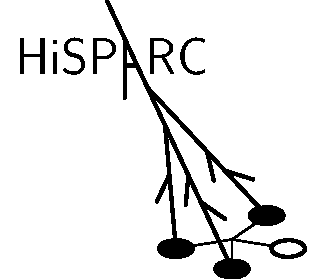
\includegraphics{logo.pdf}\par}
\renewcommand{\releasename}{Release}
\makeindex

\makeatletter
\def\PYG@reset{\let\PYG@it=\relax \let\PYG@bf=\relax%
    \let\PYG@ul=\relax \let\PYG@tc=\relax%
    \let\PYG@bc=\relax \let\PYG@ff=\relax}
\def\PYG@tok#1{\csname PYG@tok@#1\endcsname}
\def\PYG@toks#1+{\ifx\relax#1\empty\else%
    \PYG@tok{#1}\expandafter\PYG@toks\fi}
\def\PYG@do#1{\PYG@bc{\PYG@tc{\PYG@ul{%
    \PYG@it{\PYG@bf{\PYG@ff{#1}}}}}}}
\def\PYG#1#2{\PYG@reset\PYG@toks#1+\relax+\PYG@do{#2}}

\expandafter\def\csname PYG@tok@gd\endcsname{\def\PYG@tc##1{\textcolor[rgb]{0.63,0.00,0.00}{##1}}}
\expandafter\def\csname PYG@tok@gu\endcsname{\let\PYG@bf=\textbf\def\PYG@tc##1{\textcolor[rgb]{0.50,0.00,0.50}{##1}}}
\expandafter\def\csname PYG@tok@gt\endcsname{\def\PYG@tc##1{\textcolor[rgb]{0.00,0.27,0.87}{##1}}}
\expandafter\def\csname PYG@tok@gs\endcsname{\let\PYG@bf=\textbf}
\expandafter\def\csname PYG@tok@gr\endcsname{\def\PYG@tc##1{\textcolor[rgb]{1.00,0.00,0.00}{##1}}}
\expandafter\def\csname PYG@tok@cm\endcsname{\let\PYG@it=\textit\def\PYG@tc##1{\textcolor[rgb]{0.25,0.50,0.56}{##1}}}
\expandafter\def\csname PYG@tok@vg\endcsname{\def\PYG@tc##1{\textcolor[rgb]{0.73,0.38,0.84}{##1}}}
\expandafter\def\csname PYG@tok@m\endcsname{\def\PYG@tc##1{\textcolor[rgb]{0.13,0.50,0.31}{##1}}}
\expandafter\def\csname PYG@tok@mh\endcsname{\def\PYG@tc##1{\textcolor[rgb]{0.13,0.50,0.31}{##1}}}
\expandafter\def\csname PYG@tok@cs\endcsname{\def\PYG@tc##1{\textcolor[rgb]{0.25,0.50,0.56}{##1}}\def\PYG@bc##1{\setlength{\fboxsep}{0pt}\colorbox[rgb]{1.00,0.94,0.94}{\strut ##1}}}
\expandafter\def\csname PYG@tok@ge\endcsname{\let\PYG@it=\textit}
\expandafter\def\csname PYG@tok@vc\endcsname{\def\PYG@tc##1{\textcolor[rgb]{0.73,0.38,0.84}{##1}}}
\expandafter\def\csname PYG@tok@il\endcsname{\def\PYG@tc##1{\textcolor[rgb]{0.13,0.50,0.31}{##1}}}
\expandafter\def\csname PYG@tok@go\endcsname{\def\PYG@tc##1{\textcolor[rgb]{0.20,0.20,0.20}{##1}}}
\expandafter\def\csname PYG@tok@cp\endcsname{\def\PYG@tc##1{\textcolor[rgb]{0.00,0.44,0.13}{##1}}}
\expandafter\def\csname PYG@tok@gi\endcsname{\def\PYG@tc##1{\textcolor[rgb]{0.00,0.63,0.00}{##1}}}
\expandafter\def\csname PYG@tok@gh\endcsname{\let\PYG@bf=\textbf\def\PYG@tc##1{\textcolor[rgb]{0.00,0.00,0.50}{##1}}}
\expandafter\def\csname PYG@tok@ni\endcsname{\let\PYG@bf=\textbf\def\PYG@tc##1{\textcolor[rgb]{0.84,0.33,0.22}{##1}}}
\expandafter\def\csname PYG@tok@nl\endcsname{\let\PYG@bf=\textbf\def\PYG@tc##1{\textcolor[rgb]{0.00,0.13,0.44}{##1}}}
\expandafter\def\csname PYG@tok@nn\endcsname{\let\PYG@bf=\textbf\def\PYG@tc##1{\textcolor[rgb]{0.05,0.52,0.71}{##1}}}
\expandafter\def\csname PYG@tok@no\endcsname{\def\PYG@tc##1{\textcolor[rgb]{0.38,0.68,0.84}{##1}}}
\expandafter\def\csname PYG@tok@na\endcsname{\def\PYG@tc##1{\textcolor[rgb]{0.25,0.44,0.63}{##1}}}
\expandafter\def\csname PYG@tok@nb\endcsname{\def\PYG@tc##1{\textcolor[rgb]{0.00,0.44,0.13}{##1}}}
\expandafter\def\csname PYG@tok@nc\endcsname{\let\PYG@bf=\textbf\def\PYG@tc##1{\textcolor[rgb]{0.05,0.52,0.71}{##1}}}
\expandafter\def\csname PYG@tok@nd\endcsname{\let\PYG@bf=\textbf\def\PYG@tc##1{\textcolor[rgb]{0.33,0.33,0.33}{##1}}}
\expandafter\def\csname PYG@tok@ne\endcsname{\def\PYG@tc##1{\textcolor[rgb]{0.00,0.44,0.13}{##1}}}
\expandafter\def\csname PYG@tok@nf\endcsname{\def\PYG@tc##1{\textcolor[rgb]{0.02,0.16,0.49}{##1}}}
\expandafter\def\csname PYG@tok@si\endcsname{\let\PYG@it=\textit\def\PYG@tc##1{\textcolor[rgb]{0.44,0.63,0.82}{##1}}}
\expandafter\def\csname PYG@tok@s2\endcsname{\def\PYG@tc##1{\textcolor[rgb]{0.25,0.44,0.63}{##1}}}
\expandafter\def\csname PYG@tok@vi\endcsname{\def\PYG@tc##1{\textcolor[rgb]{0.73,0.38,0.84}{##1}}}
\expandafter\def\csname PYG@tok@nt\endcsname{\let\PYG@bf=\textbf\def\PYG@tc##1{\textcolor[rgb]{0.02,0.16,0.45}{##1}}}
\expandafter\def\csname PYG@tok@nv\endcsname{\def\PYG@tc##1{\textcolor[rgb]{0.73,0.38,0.84}{##1}}}
\expandafter\def\csname PYG@tok@s1\endcsname{\def\PYG@tc##1{\textcolor[rgb]{0.25,0.44,0.63}{##1}}}
\expandafter\def\csname PYG@tok@gp\endcsname{\let\PYG@bf=\textbf\def\PYG@tc##1{\textcolor[rgb]{0.78,0.36,0.04}{##1}}}
\expandafter\def\csname PYG@tok@sh\endcsname{\def\PYG@tc##1{\textcolor[rgb]{0.25,0.44,0.63}{##1}}}
\expandafter\def\csname PYG@tok@ow\endcsname{\let\PYG@bf=\textbf\def\PYG@tc##1{\textcolor[rgb]{0.00,0.44,0.13}{##1}}}
\expandafter\def\csname PYG@tok@sx\endcsname{\def\PYG@tc##1{\textcolor[rgb]{0.78,0.36,0.04}{##1}}}
\expandafter\def\csname PYG@tok@bp\endcsname{\def\PYG@tc##1{\textcolor[rgb]{0.00,0.44,0.13}{##1}}}
\expandafter\def\csname PYG@tok@c1\endcsname{\let\PYG@it=\textit\def\PYG@tc##1{\textcolor[rgb]{0.25,0.50,0.56}{##1}}}
\expandafter\def\csname PYG@tok@kc\endcsname{\let\PYG@bf=\textbf\def\PYG@tc##1{\textcolor[rgb]{0.00,0.44,0.13}{##1}}}
\expandafter\def\csname PYG@tok@c\endcsname{\let\PYG@it=\textit\def\PYG@tc##1{\textcolor[rgb]{0.25,0.50,0.56}{##1}}}
\expandafter\def\csname PYG@tok@mf\endcsname{\def\PYG@tc##1{\textcolor[rgb]{0.13,0.50,0.31}{##1}}}
\expandafter\def\csname PYG@tok@err\endcsname{\def\PYG@bc##1{\setlength{\fboxsep}{0pt}\fcolorbox[rgb]{1.00,0.00,0.00}{1,1,1}{\strut ##1}}}
\expandafter\def\csname PYG@tok@kd\endcsname{\let\PYG@bf=\textbf\def\PYG@tc##1{\textcolor[rgb]{0.00,0.44,0.13}{##1}}}
\expandafter\def\csname PYG@tok@ss\endcsname{\def\PYG@tc##1{\textcolor[rgb]{0.32,0.47,0.09}{##1}}}
\expandafter\def\csname PYG@tok@sr\endcsname{\def\PYG@tc##1{\textcolor[rgb]{0.14,0.33,0.53}{##1}}}
\expandafter\def\csname PYG@tok@mo\endcsname{\def\PYG@tc##1{\textcolor[rgb]{0.13,0.50,0.31}{##1}}}
\expandafter\def\csname PYG@tok@mi\endcsname{\def\PYG@tc##1{\textcolor[rgb]{0.13,0.50,0.31}{##1}}}
\expandafter\def\csname PYG@tok@kn\endcsname{\let\PYG@bf=\textbf\def\PYG@tc##1{\textcolor[rgb]{0.00,0.44,0.13}{##1}}}
\expandafter\def\csname PYG@tok@o\endcsname{\def\PYG@tc##1{\textcolor[rgb]{0.40,0.40,0.40}{##1}}}
\expandafter\def\csname PYG@tok@kr\endcsname{\let\PYG@bf=\textbf\def\PYG@tc##1{\textcolor[rgb]{0.00,0.44,0.13}{##1}}}
\expandafter\def\csname PYG@tok@s\endcsname{\def\PYG@tc##1{\textcolor[rgb]{0.25,0.44,0.63}{##1}}}
\expandafter\def\csname PYG@tok@kp\endcsname{\def\PYG@tc##1{\textcolor[rgb]{0.00,0.44,0.13}{##1}}}
\expandafter\def\csname PYG@tok@w\endcsname{\def\PYG@tc##1{\textcolor[rgb]{0.73,0.73,0.73}{##1}}}
\expandafter\def\csname PYG@tok@kt\endcsname{\def\PYG@tc##1{\textcolor[rgb]{0.56,0.13,0.00}{##1}}}
\expandafter\def\csname PYG@tok@sc\endcsname{\def\PYG@tc##1{\textcolor[rgb]{0.25,0.44,0.63}{##1}}}
\expandafter\def\csname PYG@tok@sb\endcsname{\def\PYG@tc##1{\textcolor[rgb]{0.25,0.44,0.63}{##1}}}
\expandafter\def\csname PYG@tok@k\endcsname{\let\PYG@bf=\textbf\def\PYG@tc##1{\textcolor[rgb]{0.00,0.44,0.13}{##1}}}
\expandafter\def\csname PYG@tok@se\endcsname{\let\PYG@bf=\textbf\def\PYG@tc##1{\textcolor[rgb]{0.25,0.44,0.63}{##1}}}
\expandafter\def\csname PYG@tok@sd\endcsname{\let\PYG@it=\textit\def\PYG@tc##1{\textcolor[rgb]{0.25,0.44,0.63}{##1}}}

\def\PYGZbs{\char`\\}
\def\PYGZus{\char`\_}
\def\PYGZob{\char`\{}
\def\PYGZcb{\char`\}}
\def\PYGZca{\char`\^}
\def\PYGZam{\char`\&}
\def\PYGZlt{\char`\<}
\def\PYGZgt{\char`\>}
\def\PYGZsh{\char`\#}
\def\PYGZpc{\char`\%}
\def\PYGZdl{\char`\$}
\def\PYGZhy{\char`\-}
\def\PYGZsq{\char`\'}
\def\PYGZdq{\char`\"}
\def\PYGZti{\char`\~}
% for compatibility with earlier versions
\def\PYGZat{@}
\def\PYGZlb{[}
\def\PYGZrb{]}
\makeatother

\begin{document}

\maketitle
\tableofcontents
\phantomsection\label{index::doc}


Servers:


\chapter{Installation of Frome}
\label{frome:welcome-to-hisparc-server-management-s-documentation}\label{frome::doc}\label{frome:installation-of-frome}
Granting davidf rights to manage software and services:

\begin{Verbatim}[commandchars=\\\{\}]
\PYG{o}{(}root\PYG{o}{)}\PYG{n+nv}{\PYGZdl{} }visudo
\end{Verbatim}

and adding:

\begin{Verbatim}[commandchars=\\\{\}]
davidf  ALL = SOFTWARE, SERVICES
\end{Verbatim}

Preparing for source install:

\begin{Verbatim}[commandchars=\\\{\}]
\PYG{o}{(}root\PYG{o}{)}\PYG{n+nv}{\PYGZdl{} }\PYG{n+nb}{cd} /usr/local/src/
\PYG{o}{(}root\PYG{o}{)}\PYG{n+nv}{\PYGZdl{} }mkdir hisparc
\PYG{o}{(}root\PYG{o}{)}\PYG{n+nv}{\PYGZdl{} }chown davidf.hisparc hisparc/
\PYG{n+nv}{\PYGZdl{} }chmod g+w hisparc/
\end{Verbatim}

In /etc/ld.so.conf.d new file usrlocal.conf, to let ldconfig find
libraries of locally installed software:

\begin{Verbatim}[commandchars=\\\{\}]
/usr/local/lib
\end{Verbatim}


\section{Python}
\label{frome:python}
Python:

\begin{Verbatim}[commandchars=\\\{\}]
\PYG{n+nv}{\PYGZdl{} }\PYG{n+nb}{cd} /usr/local/src/hisparc
\PYG{n+nv}{\PYGZdl{} }wget http://www.python.org/ftp/python/2.6.4/Python\PYGZhy{}2.6.4.tgz
\PYG{n+nv}{\PYGZdl{} }tar xvzf Python\PYGZhy{}2.6.4.tgz
\PYG{n+nv}{\PYGZdl{} }\PYG{n+nb}{cd }Python\PYGZhy{}2.6.4
\PYG{n+nv}{\PYGZdl{} }./configure \PYGZhy{}\PYGZhy{}enable\PYGZhy{}shared
\PYG{n+nv}{\PYGZdl{} }make
\PYG{o}{(}root\PYG{o}{)}\PYG{n+nv}{\PYGZdl{} }make install
\end{Verbatim}

Then, run:

\begin{Verbatim}[commandchars=\\\{\}]
\PYG{o}{(}root\PYG{o}{)}\PYG{n+nv}{\PYGZdl{} }ldconfig
\end{Verbatim}

Now, the python libraries are registered.


\section{Python Setuptools}
\label{frome:python-setuptools}
From egg:

\begin{Verbatim}[commandchars=\\\{\}]
\PYG{n+nv}{\PYGZdl{} }\PYG{n+nb}{cd} /usr/local/src/hisparc
\PYG{n+nv}{\PYGZdl{} }wget http://pypi.python.org/packages/2.6/s/setuptools/setuptools\PYGZhy{}0.6c11\PYGZhy{}py2.6.egg\PYGZsh{}md5\PYG{o}{=}bfa92100bd772d5a213eedd356d64086
\PYG{o}{(}root\PYG{o}{)}\PYG{n+nv}{\PYGZdl{} }sh setuptools\PYGZhy{}0.6c11\PYGZhy{}py2.6.egg
\end{Verbatim}


\section{IPython, an interactive Python shell}
\label{frome:ipython-an-interactive-python-shell}
Download and install IPython:

\begin{Verbatim}[commandchars=\\\{\}]
\PYG{o}{(}root\PYG{o}{)}\PYG{n+nv}{\PYGZdl{} }easy\PYGZus{}install ipython
\end{Verbatim}


\section{Web server}
\label{frome:web-server}
Install apache development libraries:

\begin{Verbatim}[commandchars=\\\{\}]
\PYG{n+nv}{\PYGZdl{} }sudo yum install httpd\PYGZhy{}devel

\PYG{o}{=}\PYG{o}{=}\PYG{o}{=}\PYG{o}{=}\PYG{o}{=}\PYG{o}{=}\PYG{o}{=}\PYG{o}{=}\PYG{o}{=}\PYG{o}{=}\PYG{o}{=}\PYG{o}{=}\PYG{o}{=}\PYG{o}{=}\PYG{o}{=}\PYG{o}{=}\PYG{o}{=}\PYG{o}{=}\PYG{o}{=}\PYG{o}{=}\PYG{o}{=}\PYG{o}{=}\PYG{o}{=}\PYG{o}{=}\PYG{o}{=}\PYG{o}{=}\PYG{o}{=}\PYG{o}{=}\PYG{o}{=}\PYG{o}{=}\PYG{o}{=}\PYG{o}{=}\PYG{o}{=}\PYG{o}{=}\PYG{o}{=}\PYG{o}{=}\PYG{o}{=}\PYG{o}{=}\PYG{o}{=}\PYG{o}{=}\PYG{o}{=}\PYG{o}{=}\PYG{o}{=}\PYG{o}{=}\PYG{o}{=}\PYG{o}{=}\PYG{o}{=}\PYG{o}{=}\PYG{o}{=}\PYG{o}{=}\PYG{o}{=}\PYG{o}{=}\PYG{o}{=}\PYG{o}{=}\PYG{o}{=}\PYG{o}{=}\PYG{o}{=}\PYG{o}{=}\PYG{o}{=}\PYG{o}{=}\PYG{o}{=}\PYG{o}{=}\PYG{o}{=}\PYG{o}{=}\PYG{o}{=}\PYG{o}{=}\PYG{o}{=}\PYG{o}{=}\PYG{o}{=}\PYG{o}{=}\PYG{o}{=}\PYG{o}{=}\PYG{o}{=}\PYG{o}{=}\PYG{o}{=}\PYG{o}{=}\PYG{o}{=}\PYG{o}{=}\PYG{o}{=}\PYG{o}{=}
 Package             Arch        Version                 Repository        \PYG{n+nv}{Size}
\PYG{o}{=}\PYG{o}{=}\PYG{o}{=}\PYG{o}{=}\PYG{o}{=}\PYG{o}{=}\PYG{o}{=}\PYG{o}{=}\PYG{o}{=}\PYG{o}{=}\PYG{o}{=}\PYG{o}{=}\PYG{o}{=}\PYG{o}{=}\PYG{o}{=}\PYG{o}{=}\PYG{o}{=}\PYG{o}{=}\PYG{o}{=}\PYG{o}{=}\PYG{o}{=}\PYG{o}{=}\PYG{o}{=}\PYG{o}{=}\PYG{o}{=}\PYG{o}{=}\PYG{o}{=}\PYG{o}{=}\PYG{o}{=}\PYG{o}{=}\PYG{o}{=}\PYG{o}{=}\PYG{o}{=}\PYG{o}{=}\PYG{o}{=}\PYG{o}{=}\PYG{o}{=}\PYG{o}{=}\PYG{o}{=}\PYG{o}{=}\PYG{o}{=}\PYG{o}{=}\PYG{o}{=}\PYG{o}{=}\PYG{o}{=}\PYG{o}{=}\PYG{o}{=}\PYG{o}{=}\PYG{o}{=}\PYG{o}{=}\PYG{o}{=}\PYG{o}{=}\PYG{o}{=}\PYG{o}{=}\PYG{o}{=}\PYG{o}{=}\PYG{o}{=}\PYG{o}{=}\PYG{o}{=}\PYG{o}{=}\PYG{o}{=}\PYG{o}{=}\PYG{o}{=}\PYG{o}{=}\PYG{o}{=}\PYG{o}{=}\PYG{o}{=}\PYG{o}{=}\PYG{o}{=}\PYG{o}{=}\PYG{o}{=}\PYG{o}{=}\PYG{o}{=}\PYG{o}{=}\PYG{o}{=}\PYG{o}{=}\PYG{o}{=}\PYG{o}{=}\PYG{o}{=}\PYG{o}{=}
Installing:
 httpd\PYGZhy{}devel         i386        2.2.3\PYGZhy{}31.sl5.2          sl\PYGZhy{}security      147 k
 httpd\PYGZhy{}devel         x86\PYGZus{}64      2.2.3\PYGZhy{}31.sl5.2          sl\PYGZhy{}security      147 k
Installing \PYG{k}{for }dependencies:
 apr                 x86\PYGZus{}64      1.2.7\PYGZhy{}11.el5\PYGZus{}3.1        sl\PYGZhy{}security      118 k
 apr\PYGZhy{}devel           x86\PYGZus{}64      1.2.7\PYGZhy{}11.el5\PYGZus{}3.1        sl\PYGZhy{}security      237 k
 apr\PYGZhy{}util            x86\PYGZus{}64      1.2.7\PYGZhy{}7.el5\PYGZus{}3.2         sl\PYGZhy{}security       74 k
 apr\PYGZhy{}util\PYGZhy{}devel      x86\PYGZus{}64      1.2.7\PYGZhy{}7.el5\PYGZus{}3.2         sl\PYGZhy{}security       53 k
 httpd               x86\PYGZus{}64      2.2.3\PYGZhy{}31.sl5.2          sl\PYGZhy{}security      1.2 M
\end{Verbatim}

Change configuration in /etc/httpd/conf/httpd.conf. Patch:

\begin{Verbatim}[commandchars=\\\{\}]
--- httpd.conf.orig     2009-12-04 14:35:39.000000000 +0100
+++ httpd.conf  2009-12-04 14:35:50.000000000 +0100
@@ -228,8 +228,8 @@
 \#  when the value of (unsigned)Group is above 60000;
 \#  don't use Group \#-1 on these systems!
 \#
-User apache
-Group apache
+User www
+Group www

 \#\#\# Section 2: 'Main' server configuration
 \#
\end{Verbatim}

Enabling httpd on startup:

\begin{Verbatim}[commandchars=\\\{\}]
\PYG{n+nv}{\PYGZdl{} }sudo /sbin/chkconfig \PYGZhy{}\PYGZhy{}add httpd
\PYG{n+nv}{\PYGZdl{} }sudo /sbin/chkconfig \PYGZhy{}\PYGZhy{}levels 35 httpd on
\end{Verbatim}

Starting httpd now:

\begin{Verbatim}[commandchars=\\\{\}]
\PYG{n+nv}{\PYGZdl{} }sudo /sbin/service httpd start
\end{Verbatim}

For mod\_wsgi:

\begin{Verbatim}[commandchars=\\\{\}]
\PYG{n+nv}{\PYGZdl{} }\PYG{n+nb}{cd} /usr/local/src/hisparc
\PYG{n+nv}{\PYGZdl{} }wget http://modwsgi.googlecode.com/files/mod\PYGZus{}wsgi\PYGZhy{}3.1.tar.gz
\PYG{n+nv}{\PYGZdl{} }tar xvzf mod\PYGZus{}wsgi\PYGZhy{}3.1.tar.gz
\PYG{n+nv}{\PYGZdl{} }\PYG{n+nb}{cd }mod\PYGZus{}wsgi\PYGZhy{}3.1
\PYG{n+nv}{\PYGZdl{} }./configure
\PYG{n+nv}{\PYGZdl{} }make
\PYG{o}{(}root\PYG{o}{)}\PYG{n+nv}{\PYGZdl{} }make install
\end{Verbatim}

Change configuration in /etc/httpd/conf/httpd.conf. Patch:

\begin{Verbatim}[commandchars=\\\{\}]
--- httpd.conf.orig     2009-12-04 15:19:01.000000000 +0100
+++ httpd.conf  2009-12-04 15:34:30.000000000 +0100
@@ -197,6 +197,7 @@
 LoadModule mem\_cache\_module modules/mod\_mem\_cache.so
 LoadModule cgi\_module modules/mod\_cgi.so
 LoadModule version\_module modules/mod\_version.so
+LoadModule wsgi\_module modules/mod\_wsgi.so

 \#
 \# The following modules are not loaded by default:
\end{Verbatim}

Restarting apache:

\begin{Verbatim}[commandchars=\\\{\}]
\PYG{n+nv}{\PYGZdl{} }sudo /sbin/service httpd restart
\end{Verbatim}


\section{Version control}
\label{frome:version-control}
Install bazaar from source:

\begin{Verbatim}[commandchars=\\\{\}]
\PYG{n+nv}{\PYGZdl{} }\PYG{n+nb}{cd} /usr/local/src/hisparc
\PYG{n+nv}{\PYGZdl{} }wget http://launchpad.net/bzr/2.0/2.0.2/+download/bzr\PYGZhy{}2.0.2.tar.gz
\PYG{n+nv}{\PYGZdl{} }tar xvzf bzr\PYGZhy{}2.0.2.tar.gz
\PYG{n+nv}{\PYGZdl{} }\PYG{n+nb}{cd }bzr\PYGZhy{}2.0.2
\PYG{o}{(}root\PYG{o}{)}\PYG{n+nv}{\PYGZdl{} }python setup.py install
\end{Verbatim}


\subsection{Paramiko}
\label{frome:paramiko}
Paramiko supports ssh2 for python, which is needed to do a checkout of our
application's sources over sftp.  Install using easy\_install:

\begin{Verbatim}[commandchars=\\\{\}]
\PYG{o}{(}root\PYG{o}{)}\PYG{n+nv}{\PYGZdl{} }easy\PYGZus{}install paramiko
\end{Verbatim}

This will automatically download, compile and install dependencies
(pycrypto).


\section{Datastore web application}
\label{frome:datastore-web-application}
The datastore application is driving our central data storage solution.
It is a pure python implementation under complete version control.


\subsection{Prerequisites}
\label{frome:prerequisites}
The datastore application uses PyTables and the underlying HDF5 library to
store binary data files.  PyTables depends heavily on NumPy.:

\begin{Verbatim}[commandchars=\\\{\}]
\PYG{o}{(}root\PYG{o}{)}\PYG{n+nv}{\PYGZdl{} }easy\PYGZus{}install numpy
\end{Verbatim}

This gives an error:

\begin{Verbatim}[commandchars=\\\{\}]
/tmp/easy\_install-JePGOA/numpy-1.4.0rc1/numpy/distutils/misc\_util.py:248: RuntimeWarning: Parent module 'numpy.distutils' not found while handling absolute import
Error in atexit.\_run\_exitfuncs:
Traceback (most recent call last):
  File "/usr/local/lib/python2.6/atexit.py", line 24, in \_run\_exitfuncs
    func(*targs, **kargs)
  File "/tmp/easy\_install-JePGOA/numpy-1.4.0rc1/numpy/distutils/misc\_util.py", line 248, in clean\_up\_temporary\_directory
ImportError: No module named numpy.distutils
Error in sys.exitfunc:
Traceback (most recent call last):
  File "/usr/local/lib/python2.6/atexit.py", line 24, in \_run\_exitfuncs
    func(*targs, **kargs)
  File "/tmp/easy\_install-JePGOA/numpy-1.4.0rc1/numpy/distutils/misc\_util.py", line 248, in clean\_up\_temporary\_directory
ImportError: No module named numpy.distutils
\end{Verbatim}

So, rerun the command, this time without errors:

\begin{Verbatim}[commandchars=\\\{\}]
\PYG{o}{(}root\PYG{o}{)}\PYG{n+nv}{\PYGZdl{} }easy\PYGZus{}install numpy
\end{Verbatim}

Now:

\begin{Verbatim}[commandchars=\\\{\}]
\PYG{n+nv}{\PYGZdl{} }\PYG{n+nb}{cd} /usr/local/src/hisparc
\PYG{n+nv}{\PYGZdl{} }wget http://www.hdfgroup.org/ftp/HDF5/prev\PYGZhy{}releases/hdf5\PYGZhy{}1.8.3/src/hdf5\PYGZhy{}1.8.3.tar.gz
\PYG{n+nv}{\PYGZdl{} }tar xvzf hdf5\PYGZhy{}1.8.3.tar.gz
\PYG{n+nv}{\PYGZdl{} }\PYG{n+nb}{cd }hdf5\PYGZhy{}1.8.3
\PYG{n+nv}{\PYGZdl{} }./configure \PYGZhy{}\PYGZhy{}prefix\PYG{o}{=}/usr/local
\PYG{n+nv}{\PYGZdl{} }make
\PYG{o}{(}root\PYG{o}{)}\PYG{n+nv}{\PYGZdl{} }make install
\PYG{o}{(}root\PYG{o}{)}\PYG{n+nv}{\PYGZdl{} }ldconfig
\end{Verbatim}

And, finally, install PyTables itself:

\begin{Verbatim}[commandchars=\\\{\}]
\PYG{o}{(}root\PYG{o}{)}\PYG{n+nv}{\PYGZdl{} }easy\PYGZus{}install tables
\end{Verbatim}


\subsection{Setting up datastore}
\label{frome:setting-up-datastore}
In summary:
\begin{itemize}
\item {} 
Created a /var/www/wsgi-bin directory from which to run the wsgi
applications

\item {} 
Created a subdirectory owned by davidf.hisparc inside this wsgi-bin

\item {} 
Did a checkout of the datastore sources inside the subdirectory

\item {} 
Made a local copy of the application into the parent (wsgi-bin) and
edited to set the correct local full path

\item {} 
Added the wsgi application to the Apache configuration

\end{itemize}

Here we go:

\begin{Verbatim}[commandchars=\\\{\}]
\PYG{o}{(}root\PYG{o}{)}\PYG{n+nv}{\PYGZdl{} }\PYG{n+nb}{cd} /var/www
\PYG{o}{(}root\PYG{o}{)}\PYG{n+nv}{\PYGZdl{} }mkdir wsgi\PYGZhy{}bin
\PYG{o}{(}root\PYG{o}{)}\PYG{n+nv}{\PYGZdl{} }\PYG{n+nb}{cd }wsgi\PYGZhy{}bin
\PYG{o}{(}root\PYG{o}{)}\PYG{n+nv}{\PYGZdl{} }mkdir datastore
\PYG{o}{(}root\PYG{o}{)}\PYG{n+nv}{\PYGZdl{} }chown davidf.hisparc datastore
\PYG{o}{(}root\PYG{o}{)}\PYG{n+nv}{\PYGZdl{} }chmod g+w datastore
\PYG{n+nv}{\PYGZdl{} }\PYG{n+nb}{cd} /var/www/wsgi\PYGZhy{}bin/datastore/
\PYG{n+nv}{\PYGZdl{} }bzr co sftp://admhispa@login.nikhef.nl/project/hisparc/bzr/datastore/trunk .
\end{Verbatim}

Copy the application.wsgi and config.ini from the examples directory:

\begin{Verbatim}[commandchars=\\\{\}]
\PYG{o}{(}root\PYG{o}{)}\PYG{n+nv}{\PYGZdl{} }\PYG{n+nb}{cd} /var/www/wsgi\PYGZhy{}bin
\PYG{o}{(}root\PYG{o}{)}\PYG{n+nv}{\PYGZdl{} }cp datastore/examples/application.wsgi datastore.wsgi
\PYG{o}{(}root\PYG{o}{)}\PYG{n+nv}{\PYGZdl{} }cp datastore/examples/config.ini datastore/
\PYG{o}{(}root\PYG{o}{)}\PYG{n+nv}{\PYGZdl{} }chown davidf.hisparc datastore.wsgi datastore/config.ini
\PYG{o}{(}root\PYG{o}{)}\PYG{n+nv}{\PYGZdl{} }chmod g+w datastore.wsgi datastore/config.ini
\end{Verbatim}

Edited /var/www/wsgi-bin/datastore.wsgi and set the correct paths:

\begin{Verbatim}[commandchars=\\\{\}]
\PYG{n}{sys}\PYG{o}{.}\PYG{n}{path}\PYG{o}{.}\PYG{n}{append}\PYG{p}{(}\PYG{l+s}{\PYGZsq{}}\PYG{l+s}{/var/www/wsgi\PYGZhy{}bin/datastore/wsgi}\PYG{l+s}{\PYGZsq{}}\PYG{p}{)}
\PYG{n}{configfile} \PYG{o}{=} \PYG{p}{(}\PYG{l+s}{\PYGZsq{}}\PYG{l+s}{/var/www/wsgi\PYGZhy{}bin/datastore/config.ini}\PYG{l+s}{\PYGZsq{}}\PYG{p}{)}
\end{Verbatim}

The config.ini now reads:

\begin{Verbatim}[commandchars=\\\{\}]
[General]
log=/var/log/hisparc/hisparc.log
loglevel=debug
station\_list=/databases/frome/station\_list.csv
data\_dir=/databases/frome

[Writer]
sleep=1
\end{Verbatim}

I had to create the appropriate directory in /var/log and grant rights:

\begin{Verbatim}[commandchars=\\\{\}]
\PYG{o}{(}root\PYG{o}{)}\PYG{n+nv}{\PYGZdl{} }\PYG{n+nb}{cd} /var/log
\PYG{o}{(}root\PYG{o}{)}\PYG{n+nv}{\PYGZdl{} }mkdir hisparc
\PYG{o}{(}root\PYG{o}{)}\PYG{n+nv}{\PYGZdl{} }chown www.hisparc hisparc
\PYG{o}{(}root\PYG{o}{)}\PYG{n+nv}{\PYGZdl{} }chmod g+w hisparc
\end{Verbatim}

Then, added datastore to the Apache configuration:

\begin{Verbatim}[commandchars=\\\{\}]
\PYG{o}{(}root\PYG{o}{)}\PYG{n+nv}{\PYGZdl{} }\PYG{n+nb}{cd} /etc/httpd/conf.d/
\PYG{o}{(}root\PYG{o}{)}\PYG{n+nv}{\PYGZdl{} }touch hisparc.conf
\PYG{o}{(}root\PYG{o}{)}\PYG{n+nv}{\PYGZdl{} }chown davidf.hisparc hisparc.conf
\PYG{o}{(}root\PYG{o}{)}\PYG{n+nv}{\PYGZdl{} }chmod g+w hisparc.conf
\end{Verbatim}

And edited hisparc.conf to contain:

\begin{Verbatim}[commandchars=\\\{\}]
\PYG{n}{WSGIScriptAlias} \PYG{o}{/}\PYG{n}{hisparc}\PYG{o}{/}\PYG{n}{upload} \PYG{o}{/}\PYG{n}{var}\PYG{o}{/}\PYG{n}{www}\PYG{o}{/}\PYG{n}{wsgi}\PYG{o}{\PYGZhy{}}\PYG{n+nb}{bin}\PYG{o}{/}\PYG{n}{datastore}\PYG{o}{.}\PYG{n}{wsgi}
\end{Verbatim}

Reload Apache configuration:

\begin{Verbatim}[commandchars=\\\{\}]
\PYG{n+nv}{\PYGZdl{} }sudo /sbin/service httpd reload
\end{Verbatim}


\section{TODO}
\label{frome:todo}
Writer app!


\section{(Maybe) Not relevant}
\label{frome:maybe-not-relevant}
install: yum-utils
easy\_install dozer
easy\_install pil (requirement of dozer)
easy\_install mysql-python (for migration)
install: gcc-gfortran
easy\_install virtualenvwrapper
install: blas-devel lapack-devel (for scipy)


\chapter{Installation of Pique}
\label{pique:installation-of-pique}\label{pique::doc}
Granting davidf rights to manage software and services:

\begin{Verbatim}[commandchars=\\\{\}]
\PYG{o}{(}root\PYG{o}{)}\PYG{n+nv}{\PYGZdl{} }visudo
\end{Verbatim}

and adding:

\begin{Verbatim}[commandchars=\\\{\}]
davidf  ALL = SOFTWARE, SERVICES
\end{Verbatim}

Preparing for source install:

\begin{Verbatim}[commandchars=\\\{\}]
\PYG{o}{(}root\PYG{o}{)}\PYG{n+nv}{\PYGZdl{} }\PYG{n+nb}{cd} /localstore
\PYG{o}{(}root\PYG{o}{)}\PYG{n+nv}{\PYGZdl{} }mkdir \PYGZhy{}p usr/local
\PYG{o}{(}root\PYG{o}{)}\PYG{n+nv}{\PYGZdl{} }mv /usr/local/src usr/local
\PYG{o}{(}root\PYG{o}{)}\PYG{n+nv}{\PYGZdl{} }\PYG{n+nb}{cd} /usr/local
\PYG{o}{(}root\PYG{o}{)}\PYG{n+nv}{\PYGZdl{} }ln \PYGZhy{}s /localstore/usr/local/src .
\PYG{o}{(}root\PYG{o}{)}\PYG{n+nv}{\PYGZdl{} }\PYG{n+nb}{cd} /usr/local/src/
\PYG{o}{(}root\PYG{o}{)}\PYG{n+nv}{\PYGZdl{} }mkdir hisparc
\PYG{o}{(}root\PYG{o}{)}\PYG{n+nv}{\PYGZdl{} }chown davidf.hisparc hisparc/
\PYG{n+nv}{\PYGZdl{} }chmod g+w hisparc/
\end{Verbatim}

In /etc/ld.so.conf.d new file usrlocal.conf, to let ldconfig find
libraries of locally installed software:

\begin{Verbatim}[commandchars=\\\{\}]
/usr/local/lib
\end{Verbatim}


\section{Python}
\label{pique:python}
Python:

\begin{Verbatim}[commandchars=\\\{\}]
\PYG{n+nv}{\PYGZdl{} }\PYG{n+nb}{cd} /usr/local/src/hisparc
\PYG{n+nv}{\PYGZdl{} }wget http://www.python.org/ftp/python/2.6.4/Python\PYGZhy{}2.6.4.tgz
\PYG{n+nv}{\PYGZdl{} }tar xvzf Python\PYGZhy{}2.6.4.tgz
\PYG{n+nv}{\PYGZdl{} }\PYG{n+nb}{cd }Python\PYGZhy{}2.6.4
\PYG{n+nv}{\PYGZdl{} }./configure \PYGZhy{}\PYGZhy{}enable\PYGZhy{}shared
\PYG{n+nv}{\PYGZdl{} }make
\PYG{o}{(}root\PYG{o}{)}\PYG{n+nv}{\PYGZdl{} }make install
\end{Verbatim}

Then, run:

\begin{Verbatim}[commandchars=\\\{\}]
\PYG{o}{(}root\PYG{o}{)}\PYG{n+nv}{\PYGZdl{} }ldconfig
\end{Verbatim}

Now, the python libraries are registered.


\section{Python Setuptools}
\label{pique:python-setuptools}
From egg:

\begin{Verbatim}[commandchars=\\\{\}]
\PYG{n+nv}{\PYGZdl{} }\PYG{n+nb}{cd} /usr/local/src/hisparc
\PYG{n+nv}{\PYGZdl{} }wget http://pypi.python.org/packages/2.6/s/setuptools/setuptools\PYGZhy{}0.6c11\PYGZhy{}py2.6.egg\PYGZsh{}md5\PYG{o}{=}bfa92100bd772d5a213eedd356d64086
\PYG{o}{(}root\PYG{o}{)}\PYG{n+nv}{\PYGZdl{} }sh setuptools\PYGZhy{}0.6c11\PYGZhy{}py2.6.egg
\end{Verbatim}


\section{IPython, an interactive Python shell}
\label{pique:ipython-an-interactive-python-shell}
Download and install IPython:

\begin{Verbatim}[commandchars=\\\{\}]
\PYG{o}{(}root\PYG{o}{)}\PYG{n+nv}{\PYGZdl{} }easy\PYGZus{}install ipython
\end{Verbatim}


\section{Web server}
\label{pique:web-server}
Install apache development libraries:

\begin{Verbatim}[commandchars=\\\{\}]
\PYG{n+nv}{\PYGZdl{} }sudo yum install httpd\PYGZhy{}devel

\PYG{o}{=}\PYG{o}{=}\PYG{o}{=}\PYG{o}{=}\PYG{o}{=}\PYG{o}{=}\PYG{o}{=}\PYG{o}{=}\PYG{o}{=}\PYG{o}{=}\PYG{o}{=}\PYG{o}{=}\PYG{o}{=}\PYG{o}{=}\PYG{o}{=}\PYG{o}{=}\PYG{o}{=}\PYG{o}{=}\PYG{o}{=}\PYG{o}{=}\PYG{o}{=}\PYG{o}{=}\PYG{o}{=}\PYG{o}{=}\PYG{o}{=}\PYG{o}{=}\PYG{o}{=}\PYG{o}{=}\PYG{o}{=}\PYG{o}{=}\PYG{o}{=}\PYG{o}{=}\PYG{o}{=}\PYG{o}{=}\PYG{o}{=}\PYG{o}{=}\PYG{o}{=}\PYG{o}{=}\PYG{o}{=}\PYG{o}{=}\PYG{o}{=}\PYG{o}{=}\PYG{o}{=}\PYG{o}{=}\PYG{o}{=}\PYG{o}{=}\PYG{o}{=}\PYG{o}{=}\PYG{o}{=}\PYG{o}{=}\PYG{o}{=}\PYG{o}{=}\PYG{o}{=}\PYG{o}{=}\PYG{o}{=}\PYG{o}{=}\PYG{o}{=}\PYG{o}{=}\PYG{o}{=}\PYG{o}{=}\PYG{o}{=}\PYG{o}{=}\PYG{o}{=}\PYG{o}{=}\PYG{o}{=}\PYG{o}{=}\PYG{o}{=}\PYG{o}{=}\PYG{o}{=}\PYG{o}{=}\PYG{o}{=}\PYG{o}{=}\PYG{o}{=}\PYG{o}{=}\PYG{o}{=}\PYG{o}{=}\PYG{o}{=}\PYG{o}{=}\PYG{o}{=}\PYG{o}{=}
 Package             Arch        Version                 Repository        \PYG{n+nv}{Size}
\PYG{o}{=}\PYG{o}{=}\PYG{o}{=}\PYG{o}{=}\PYG{o}{=}\PYG{o}{=}\PYG{o}{=}\PYG{o}{=}\PYG{o}{=}\PYG{o}{=}\PYG{o}{=}\PYG{o}{=}\PYG{o}{=}\PYG{o}{=}\PYG{o}{=}\PYG{o}{=}\PYG{o}{=}\PYG{o}{=}\PYG{o}{=}\PYG{o}{=}\PYG{o}{=}\PYG{o}{=}\PYG{o}{=}\PYG{o}{=}\PYG{o}{=}\PYG{o}{=}\PYG{o}{=}\PYG{o}{=}\PYG{o}{=}\PYG{o}{=}\PYG{o}{=}\PYG{o}{=}\PYG{o}{=}\PYG{o}{=}\PYG{o}{=}\PYG{o}{=}\PYG{o}{=}\PYG{o}{=}\PYG{o}{=}\PYG{o}{=}\PYG{o}{=}\PYG{o}{=}\PYG{o}{=}\PYG{o}{=}\PYG{o}{=}\PYG{o}{=}\PYG{o}{=}\PYG{o}{=}\PYG{o}{=}\PYG{o}{=}\PYG{o}{=}\PYG{o}{=}\PYG{o}{=}\PYG{o}{=}\PYG{o}{=}\PYG{o}{=}\PYG{o}{=}\PYG{o}{=}\PYG{o}{=}\PYG{o}{=}\PYG{o}{=}\PYG{o}{=}\PYG{o}{=}\PYG{o}{=}\PYG{o}{=}\PYG{o}{=}\PYG{o}{=}\PYG{o}{=}\PYG{o}{=}\PYG{o}{=}\PYG{o}{=}\PYG{o}{=}\PYG{o}{=}\PYG{o}{=}\PYG{o}{=}\PYG{o}{=}\PYG{o}{=}\PYG{o}{=}\PYG{o}{=}\PYG{o}{=}
Installing:
 httpd\PYGZhy{}devel         i386        2.2.3\PYGZhy{}31.sl5.2          sl\PYGZhy{}security      147 k
 httpd\PYGZhy{}devel         x86\PYGZus{}64      2.2.3\PYGZhy{}31.sl5.2          sl\PYGZhy{}security      147 k
Installing \PYG{k}{for }dependencies:
 apr                 x86\PYGZus{}64      1.2.7\PYGZhy{}11.el5\PYGZus{}3.1        sl\PYGZhy{}security      118 k
 apr\PYGZhy{}devel           x86\PYGZus{}64      1.2.7\PYGZhy{}11.el5\PYGZus{}3.1        sl\PYGZhy{}security      237 k
 apr\PYGZhy{}util            x86\PYGZus{}64      1.2.7\PYGZhy{}7.el5\PYGZus{}3.2         sl\PYGZhy{}security       74 k
 apr\PYGZhy{}util\PYGZhy{}devel      x86\PYGZus{}64      1.2.7\PYGZhy{}7.el5\PYGZus{}3.2         sl\PYGZhy{}security       53 k
 httpd               x86\PYGZus{}64      2.2.3\PYGZhy{}31.sl5.2          sl\PYGZhy{}security      1.2 M
\end{Verbatim}

Change configuration in /etc/httpd/conf/httpd.conf. Patch:

\begin{Verbatim}[commandchars=\\\{\}]
--- httpd.conf.orig     2009-12-04 14:35:39.000000000 +0100
+++ httpd.conf  2009-12-04 14:35:50.000000000 +0100
@@ -228,8 +228,8 @@
 \#  when the value of (unsigned)Group is above 60000;
 \#  don't use Group \#-1 on these systems!
 \#
-User apache
-Group apache
+User www
+Group www

 \#\#\# Section 2: 'Main' server configuration
 \#
\end{Verbatim}

Enabling httpd on startup:

\begin{Verbatim}[commandchars=\\\{\}]
\PYG{n+nv}{\PYGZdl{} }sudo /sbin/chkconfig \PYGZhy{}\PYGZhy{}add httpd
\PYG{n+nv}{\PYGZdl{} }sudo /sbin/chkconfig \PYGZhy{}\PYGZhy{}levels 35 httpd on
\end{Verbatim}

Starting httpd now:

\begin{Verbatim}[commandchars=\\\{\}]
\PYG{n+nv}{\PYGZdl{} }sudo /sbin/service httpd start
\end{Verbatim}

For mod\_wsgi:

\begin{Verbatim}[commandchars=\\\{\}]
\PYG{n+nv}{\PYGZdl{} }\PYG{n+nb}{cd} /usr/local/src/hisparc
\PYG{n+nv}{\PYGZdl{} }wget http://modwsgi.googlecode.com/files/mod\PYGZus{}wsgi\PYGZhy{}3.1.tar.gz
\PYG{n+nv}{\PYGZdl{} }tar xvzf mod\PYGZus{}wsgi\PYGZhy{}3.1.tar.gz
\PYG{n+nv}{\PYGZdl{} }\PYG{n+nb}{cd }mod\PYGZus{}wsgi\PYGZhy{}3.1
\PYG{n+nv}{\PYGZdl{} }./configure
\PYG{n+nv}{\PYGZdl{} }make
\PYG{o}{(}root\PYG{o}{)}\PYG{n+nv}{\PYGZdl{} }make install
\end{Verbatim}

Change configuration in /etc/httpd/conf/httpd.conf. Patch:

\begin{Verbatim}[commandchars=\\\{\}]
--- httpd.conf.orig     2009-12-04 15:19:01.000000000 +0100
+++ httpd.conf  2009-12-04 15:34:30.000000000 +0100
@@ -197,6 +197,7 @@
 LoadModule mem\_cache\_module modules/mod\_mem\_cache.so
 LoadModule cgi\_module modules/mod\_cgi.so
 LoadModule version\_module modules/mod\_version.so
+LoadModule wsgi\_module modules/mod\_wsgi.so

 \#
 \# The following modules are not loaded by default:
\end{Verbatim}

Restarting apache:

\begin{Verbatim}[commandchars=\\\{\}]
\PYG{n+nv}{\PYGZdl{} }sudo /sbin/service httpd restart
\end{Verbatim}


\section{Version control}
\label{pique:version-control}
Install bazaar from source:

\begin{Verbatim}[commandchars=\\\{\}]
\PYG{n+nv}{\PYGZdl{} }\PYG{n+nb}{cd} /usr/local/src/hisparc
\PYG{n+nv}{\PYGZdl{} }wget http://launchpad.net/bzr/2.0/2.0.2/+download/bzr\PYGZhy{}2.0.2.tar.gz
\PYG{n+nv}{\PYGZdl{} }tar xvzf bzr\PYGZhy{}2.0.2.tar.gz
\PYG{n+nv}{\PYGZdl{} }\PYG{n+nb}{cd }bzr\PYGZhy{}2.0.2
\PYG{o}{(}root\PYG{o}{)}\PYG{n+nv}{\PYGZdl{} }python setup.py install
\end{Verbatim}


\subsection{Paramiko}
\label{pique:paramiko}
Paramiko supports ssh2 for python, which is needed to do a checkout of our
application's sources over sftp.  Install using easy\_install:

\begin{Verbatim}[commandchars=\\\{\}]
\PYG{o}{(}root\PYG{o}{)}\PYG{n+nv}{\PYGZdl{} }easy\PYGZus{}install paramiko
\end{Verbatim}

This will automatically download, compile and install dependencies
(pycrypto).


\section{Public database web application}
\label{pique:public-database-web-application}
The public database blablabla.
It is a pure python implementation under complete version control.


\subsection{Prerequisites}
\label{pique:prerequisites}
The public database application uses PyTables and the underlying HDF5
library to read binary data files.  PyTables depends heavily on NumPy.:

\begin{Verbatim}[commandchars=\\\{\}]
\PYG{o}{(}root\PYG{o}{)}\PYG{n+nv}{\PYGZdl{} }easy\PYGZus{}install numpy
\end{Verbatim}

This gives an error:

\begin{Verbatim}[commandchars=\\\{\}]
/tmp/easy\_install-JePGOA/numpy-1.4.0rc1/numpy/distutils/misc\_util.py:248: RuntimeWarning: Parent module 'numpy.distutils' not found while handling absolute import
Error in atexit.\_run\_exitfuncs:
Traceback (most recent call last):
  File "/usr/local/lib/python2.6/atexit.py", line 24, in \_run\_exitfuncs
    func(*targs, **kargs)
  File "/tmp/easy\_install-JePGOA/numpy-1.4.0rc1/numpy/distutils/misc\_util.py", line 248, in clean\_up\_temporary\_directory
ImportError: No module named numpy.distutils
Error in sys.exitfunc:
Traceback (most recent call last):
  File "/usr/local/lib/python2.6/atexit.py", line 24, in \_run\_exitfuncs
    func(*targs, **kargs)
  File "/tmp/easy\_install-JePGOA/numpy-1.4.0rc1/numpy/distutils/misc\_util.py", line 248, in clean\_up\_temporary\_directory
ImportError: No module named numpy.distutils
\end{Verbatim}

So, rerun the command, this time without errors:

\begin{Verbatim}[commandchars=\\\{\}]
\PYG{o}{(}root\PYG{o}{)}\PYG{n+nv}{\PYGZdl{} }easy\PYGZus{}install numpy
\end{Verbatim}

Now:

\begin{Verbatim}[commandchars=\\\{\}]
\PYG{n+nv}{\PYGZdl{} }\PYG{n+nb}{cd} /usr/local/src/hisparc
\PYG{n+nv}{\PYGZdl{} }wget http://www.hdfgroup.org/ftp/HDF5/prev\PYGZhy{}releases/hdf5\PYGZhy{}1.8.3/src/hdf5\PYGZhy{}1.8.3.tar.gz
\PYG{n+nv}{\PYGZdl{} }tar xvzf hdf5\PYGZhy{}1.8.3.tar.gz
\PYG{n+nv}{\PYGZdl{} }\PYG{n+nb}{cd }hdf5\PYGZhy{}1.8.3
\PYG{n+nv}{\PYGZdl{} }./configure \PYGZhy{}\PYGZhy{}prefix\PYG{o}{=}/usr/local
\PYG{n+nv}{\PYGZdl{} }make
\PYG{o}{(}root\PYG{o}{)}\PYG{n+nv}{\PYGZdl{} }make install
\PYG{o}{(}root\PYG{o}{)}\PYG{n+nv}{\PYGZdl{} }ldconfig
\end{Verbatim}

And, finally, install PyTables itself:

\begin{Verbatim}[commandchars=\\\{\}]
\PYG{o}{(}root\PYG{o}{)}\PYG{n+nv}{\PYGZdl{} }easy\PYGZus{}install tables
\end{Verbatim}

The public databases graphing capabilities come from Enthought Chaco, a
python plotting library.  It needs swig to build.  Install with:

\begin{Verbatim}[commandchars=\\\{\}]
\PYG{n+nv}{\PYGZdl{} }wget http://prdownloads.sourceforge.net/swig/swig\PYGZhy{}1.3.40.tar.gz
\PYG{n+nv}{\PYGZdl{} }tar xvzf swig\PYGZhy{}1.3.40.tar.gz
\PYG{n+nv}{\PYGZdl{} }\PYG{n+nb}{cd }swig\PYGZhy{}1.3.40
\PYG{n+nv}{\PYGZdl{} }./configure
\PYG{n+nv}{\PYGZdl{} }make
\PYG{o}{(}root\PYG{o}{)}\PYG{n+nv}{\PYGZdl{} }make install
\end{Verbatim}

It also needs a GUI toolkit, like wxPython:

\begin{Verbatim}[commandchars=\\\{\}]
\PYG{n+nv}{\PYGZdl{} }wget http://downloads.sourceforge.net/wxpython/wxPython\PYGZhy{}src\PYGZhy{}2.8.10.1.tar.bz2
\PYG{n+nv}{\PYGZdl{} }tar xvjf wxPython\PYGZhy{}src\PYGZhy{}2.8.10.1.tar.bz2
\PYG{n+nv}{\PYGZdl{} }\PYG{n+nb}{cd }wxPython\PYGZhy{}src\PYGZhy{}2.8.10.1
\PYG{n+nv}{\PYGZdl{} }./configure \PYGZhy{}\PYGZhy{}enable\PYGZhy{}unicode \PYGZhy{}\PYGZhy{}with\PYGZhy{}opengl
\PYG{n+nv}{\PYGZdl{} }make \PYG{o}{\PYGZam{}\PYGZam{}} make \PYGZhy{}C contrib/src/gizmos \PYG{o}{\PYGZam{}\PYGZam{}} make \PYGZhy{}C contrib/src/stc
\PYG{o}{(}root\PYG{o}{)}\PYG{n+nv}{\PYGZdl{} }make install \PYG{o}{\PYGZam{}\PYGZam{}} make \PYGZhy{}C contrib/src/gizmos install \PYG{o}{\PYGZam{}\PYGZam{}} make \PYGZhy{}C contrib/src/stc install
\PYG{n+nv}{\PYGZdl{} }\PYG{n+nb}{cd }wxPython/src/gtk
\PYG{n+nv}{\PYGZdl{} }patch \PYGZlt{} /usr/local/src/hisparc/gdi.patch
\PYG{n+nv}{\PYGZdl{} }\PYG{n+nb}{cd} ../..
\PYG{o}{(}root\PYG{o}{)}\PYG{n+nv}{\PYGZdl{} }python setup.py install
\end{Verbatim}

The contents of the aforementioned gdi.patch is:

\begin{Verbatim}[commandchars=\\\{\}]
--- wxPython/src/gtk/\_gdi\_wrap.cpp.orig 2009-08-08 16:26:48.000000000 +0200
+++ wxPython/src/gtk/\_gdi\_wrap.cpp      2009-08-08 16:32:50.000000000 +0200
@@ -4195,6 +4195,10 @@
     virtual wxGraphicsBrush CreateRadialGradientBrush(wxDouble , wxDouble , wxDouble , wxDouble , wxDouble ,
                                                       const wxColour \&, const wxColour \&)  \PYGZob{} return wxNullGraphicsBrush; \PYGZcb{}
     virtual wxGraphicsFont CreateFont( const wxFont \& , const wxColour \& ) \PYGZob{} return wxNullGraphicsFont; \PYGZcb{}
+
+    // patch required as explained in
+    // http://groups.google.com/group/wxPython-users/browse\_thread/thread/129ba27e2f868c3c?pli=1
+    wxGraphicsBitmap CreateBitmap( const wxBitmap \&bitmap ) const \PYGZob{} return wxNullGraphicsBitmap; \PYGZcb{}
 \PYGZcb{};
\end{Verbatim}

We currently run Chaco straight out of the subversion repository.  Once a
new release has been finalized, we might go back to simply install from
PyPI.  Now, however, we have to issue:

\begin{Verbatim}[commandchars=\\\{\}]
\PYG{o}{(}root\PYG{o}{)}\PYG{n+nv}{\PYGZdl{} }easy\PYGZus{}install etsprojecttools
\PYG{n+nv}{\PYGZdl{} }ets co Chaco
\PYG{o}{(}root\PYG{o}{)}\PYG{n+nv}{\PYGZdl{} }ets install Chaco\PYGZus{}3.2.1
\end{Verbatim}


\subsection{Setting up the public database}
\label{pique:setting-up-the-public-database}
In summary:

Here we go:

\begin{Verbatim}[commandchars=\\\{\}]
\PYG{n+nv}{\PYGZdl{} }\PYG{n+nb}{cd} /usr/local/src/hisparc
\PYG{n+nv}{\PYGZdl{} }bzr co sftp://admhispa@login.nikhef.nl/project/hisparc/bzr/publicdb/trunk publicdb
\PYG{o}{(}root\PYG{o}{)}\PYG{n+nv}{\PYGZdl{} }\PYG{n+nb}{cd} /var/www
\PYG{o}{(}root\PYG{o}{)}\PYG{n+nv}{\PYGZdl{} }mkdir django\PYGZus{}publicdb
\PYG{o}{(}root\PYG{o}{)}\PYG{n+nv}{\PYGZdl{} }chown davidf.hisparc django\PYGZus{}publicdb/
\PYG{n+nv}{\PYGZdl{} }ln \PYGZhy{}s /usr/local/src/hisparc/publicdb/django\PYGZus{}publicdb/* .
\PYG{n+nv}{\PYGZdl{} }cp \PYGZhy{}\PYGZhy{}remove\PYGZhy{}destination /usr/local/src/hisparc/publicdb/django\PYGZus{}publicdb/settings.py .
\PYG{n+nv}{\PYGZdl{} }cp \PYGZhy{}\PYGZhy{}remove\PYGZhy{}destination /usr/local/src/hisparc/publicdb/django\PYGZus{}publicdb/manage.py .
\PYG{n+nv}{\PYGZdl{} }cp /usr/local/src/hisparc/publicdb/examples/django.wsgi .
\end{Verbatim}

And edit django.wsgi so that it contains the right system path:

\begin{Verbatim}[commandchars=\\\{\}]
\PYG{n}{sys}\PYG{o}{.}\PYG{n}{path}\PYG{o}{.}\PYG{n}{append}\PYG{p}{(}\PYG{l+s}{\PYGZsq{}}\PYG{l+s}{/var/www}\PYG{l+s}{\PYGZsq{}}\PYG{p}{)}
\end{Verbatim}

Then, added the public database to the Apache configuration:

\begin{Verbatim}[commandchars=\\\{\}]
\PYG{o}{(}root\PYG{o}{)}\PYG{n+nv}{\PYGZdl{} }\PYG{n+nb}{cd} /etc/httpd/conf.d/
\PYG{o}{(}root\PYG{o}{)}\PYG{n+nv}{\PYGZdl{} }touch hisparc.conf
\PYG{o}{(}root\PYG{o}{)}\PYG{n+nv}{\PYGZdl{} }chown davidf.hisparc hisparc.conf
\PYG{o}{(}root\PYG{o}{)}\PYG{n+nv}{\PYGZdl{} }chmod g+w hisparc.conf
\end{Verbatim}

And edit hisparc.conf to contain:

\begin{Verbatim}[commandchars=\\\{\}]
RedirectMatch \textasciicircum{}/\$ http://data.hisparc.nl/django/

WSGIScriptAlias /django /var/www/django\_publicdb/django.wsgi
WSGIPythonEggs /tmp

Alias /django/media /usr/local/lib/python2.6/site-packages/Django-1.1.1-py2.6.egg/django/contrib/admin/media
\end{Verbatim}

Reload Apache configuration:

\begin{Verbatim}[commandchars=\\\{\}]
\PYG{n+nv}{\PYGZdl{} }sudo /sbin/service httpd reload
\end{Verbatim}


\section{TODO}
\label{pique:todo}
South.

\begin{Verbatim}[commandchars=\\\{\}]
mkdir /var/www/media
chown www.www media
ln \PYGZhy{}s /var/www/django\PYGZus{}publicdb/static media

\PYG{n+nb}{cd} /usr/local/bin
cp /usr/local/src/hisparc/publicdb/examples/django\PYGZhy{}cron.py hisparc\PYGZhy{}update

\PYG{c}{\PYGZsh{} Run a daily check for new events, but it \PYGZus{}must\PYGZus{} be a few hours after}
\PYG{c}{\PYGZsh{} midnight, so don\PYGZsq{}t place this script in cron.daily, just to be sure.}
0 4 * * * root /usr/local/bin/hisparc\PYGZhy{}update

python PIL

django cron script on pique, changed a bit?
\end{Verbatim}


\chapter{Installation of Tietar}
\label{tietar::doc}\label{tietar:installation-of-tietar}
\begin{notice}{note}{Note:}
New nagios.cfg config and postfix config, template.cfg,
shorewall rules
\end{notice}

This server was originally installed by Tristan in May 2008.  Only
recently did David start making changes to the system.  Later changes are
documented here.  Hopefully, they will be expanded to include a
description of the complete system.

Due to a partial disk crash February 18th, 2010, we reinstalled the
system.  Due to lack of time, a lot of the original configuration was
retrieved from backups without analyzing the design.


\section{Installation}
\label{tietar:installation}
Adding user davidf:

\begin{Verbatim}[commandchars=\\\{\}]
\PYG{o}{(}root\PYG{o}{)}\PYG{n+nv}{\PYGZdl{} }adduser davidf
\PYG{o}{(}root\PYG{o}{)}\PYG{n+nv}{\PYGZdl{} }passwd davidf
\end{Verbatim}

Granting davidf rights to manage software and services:

\begin{Verbatim}[commandchars=\\\{\}]
\PYG{o}{(}root\PYG{o}{)}\PYG{n+nv}{\PYGZdl{} }visudo
\end{Verbatim}

and adding:

\begin{Verbatim}[commandchars=\\\{\}]
davidf  ALL = SOFTWARE, SERVICES
\end{Verbatim}


\section{Adding the hisparc group}
\label{tietar:adding-the-hisparc-group}
We've added the hisparc group to the system and made a few users part of it:

\begin{Verbatim}[commandchars=\\\{\}]
\PYG{o}{(}root\PYG{o}{)}\PYG{n+nv}{\PYGZdl{} }groupadd hisparc
\PYG{o}{(}root\PYG{o}{)}\PYG{n+nv}{\PYGZdl{} }usermod \PYGZhy{}G hisparc davidf
\end{Verbatim}


\section{Preparing for source install}
\label{tietar:preparing-for-source-install}
Issue:

\begin{Verbatim}[commandchars=\\\{\}]
\PYG{o}{(}root\PYG{o}{)}\PYG{n+nv}{\PYGZdl{} }\PYG{n+nb}{cd} /usr/local/src/
\PYG{o}{(}root\PYG{o}{)}\PYG{n+nv}{\PYGZdl{} }mkdir hisparc
\PYG{o}{(}root\PYG{o}{)}\PYG{n+nv}{\PYGZdl{} }chown davidf.hisparc hisparc/
\PYG{n+nv}{\PYGZdl{} }chmod g+sw hisparc/
\end{Verbatim}

In /etc/ld.so.conf.d new file usrlocal.conf, to let ldconfig find
libraries of locally installed software:

\begin{Verbatim}[commandchars=\\\{\}]
/usr/local/lib
\end{Verbatim}

Then, install a compiler:

\begin{Verbatim}[commandchars=\\\{\}]
\PYG{n+nv}{\PYGZdl{} }sudo yum install gcc
\end{Verbatim}


\section{Setting up RPMForge}
\label{tietar:setting-up-rpmforge}
RPMForge provides extra packages for CentOS, including Nagios and more
recent versions of the SSL libraries.  To enable it:

\begin{Verbatim}[commandchars=\\\{\}]
\PYG{n+nv}{\PYGZdl{} }\PYG{n+nb}{cd} /usr/local/src/hisparc
\PYG{n+nv}{\PYGZdl{} }wget http://packages.sw.be/rpmforge\PYGZhy{}release/rpmforge\PYGZhy{}release\PYGZhy{}0.5.1\PYGZhy{}1.el5.rf.i386.rpm
\PYG{n+nv}{\PYGZdl{} }sudo rpm \PYGZhy{}\PYGZhy{}import http://dag.wieers.com/rpm/packages/RPM\PYGZhy{}GPG\PYGZhy{}KEY.dag.txt
\PYG{n+nv}{\PYGZdl{} }rpm \PYGZhy{}K rpmforge\PYGZhy{}release\PYGZhy{}0.5.1\PYGZhy{}1.el5.rf.*.rpm
\PYG{n+nv}{\PYGZdl{} }sudo rpm \PYGZhy{}i rpmforge\PYGZhy{}release\PYGZhy{}0.5.1\PYGZhy{}1.el5.rf.*.rpm
\end{Verbatim}

Check succesful installation with and update packages:

\begin{Verbatim}[commandchars=\\\{\}]
\$ sudo yum check-update
\$ sudo yum update
\end{Verbatim}


\section{Python}
\label{tietar:python}
Prerequisites for standard libraries:

\begin{Verbatim}[commandchars=\\\{\}]
\PYG{n+nv}{\PYGZdl{} }sudo yum install zlib\PYGZhy{}devel
\PYG{n+nv}{\PYGZdl{} }sudo yum install bzip2\PYGZhy{}devel
\end{Verbatim}

Python:

\begin{Verbatim}[commandchars=\\\{\}]
\PYG{n+nv}{\PYGZdl{} }\PYG{n+nb}{cd} /usr/local/src/hisparc
\PYG{n+nv}{\PYGZdl{} }wget http://www.python.org/ftp/python/2.6.4/Python\PYGZhy{}2.6.4.tgz
\PYG{n+nv}{\PYGZdl{} }tar xvzf Python\PYGZhy{}2.6.4.tgz
\PYG{n+nv}{\PYGZdl{} }\PYG{n+nb}{cd }Python\PYGZhy{}2.6.4
\PYG{n+nv}{\PYGZdl{} }./configure \PYGZhy{}\PYGZhy{}enable\PYGZhy{}shared
\PYG{n+nv}{\PYGZdl{} }make
\PYG{o}{(}root\PYG{o}{)}\PYG{n+nv}{\PYGZdl{} }make install
\end{Verbatim}

Then, run:

\begin{Verbatim}[commandchars=\\\{\}]
\PYG{o}{(}root\PYG{o}{)}\PYG{n+nv}{\PYGZdl{} }ldconfig
\end{Verbatim}

Now, the python libraries are registered.


\section{Python Setuptools}
\label{tietar:python-setuptools}
From egg:

\begin{Verbatim}[commandchars=\\\{\}]
\PYG{n+nv}{\PYGZdl{} }\PYG{n+nb}{cd} /usr/local/src/hisparc
\PYG{n+nv}{\PYGZdl{} }wget http://pypi.python.org/packages/2.6/s/setuptools/setuptools\PYGZhy{}0.6c11\PYGZhy{}py2.6.egg\PYGZsh{}md5\PYG{o}{=}bfa92100bd772d5a213eedd356d64086
\PYG{o}{(}root\PYG{o}{)}\PYG{n+nv}{\PYGZdl{} }sh setuptools\PYGZhy{}0.6c11\PYGZhy{}py2.6.egg
\end{Verbatim}


\section{Web server}
\label{tietar:web-server}
Install apache:

\begin{Verbatim}[commandchars=\\\{\}]
\PYG{n+nv}{\PYGZdl{} }sudo yum install \PYG{n+nv}{httpd}

\PYG{o}{=}\PYG{o}{=}\PYG{o}{=}\PYG{o}{=}\PYG{o}{=}\PYG{o}{=}\PYG{o}{=}\PYG{o}{=}\PYG{o}{=}\PYG{o}{=}\PYG{o}{=}\PYG{o}{=}\PYG{o}{=}\PYG{o}{=}\PYG{o}{=}\PYG{o}{=}\PYG{o}{=}\PYG{o}{=}\PYG{o}{=}\PYG{o}{=}\PYG{o}{=}\PYG{o}{=}\PYG{o}{=}\PYG{o}{=}\PYG{o}{=}\PYG{o}{=}\PYG{o}{=}\PYG{o}{=}\PYG{o}{=}\PYG{o}{=}\PYG{o}{=}\PYG{o}{=}\PYG{o}{=}\PYG{o}{=}\PYG{o}{=}\PYG{o}{=}\PYG{o}{=}\PYG{o}{=}\PYG{o}{=}\PYG{o}{=}\PYG{o}{=}\PYG{o}{=}\PYG{o}{=}\PYG{o}{=}\PYG{o}{=}\PYG{o}{=}\PYG{o}{=}\PYG{o}{=}\PYG{o}{=}\PYG{o}{=}\PYG{o}{=}\PYG{o}{=}\PYG{o}{=}\PYG{o}{=}\PYG{o}{=}\PYG{o}{=}\PYG{o}{=}\PYG{o}{=}\PYG{o}{=}\PYG{o}{=}\PYG{o}{=}\PYG{o}{=}\PYG{o}{=}\PYG{o}{=}\PYG{o}{=}\PYG{o}{=}\PYG{o}{=}\PYG{o}{=}\PYG{o}{=}\PYG{o}{=}\PYG{o}{=}\PYG{o}{=}\PYG{o}{=}\PYG{o}{=}\PYG{o}{=}\PYG{o}{=}\PYG{o}{=}\PYG{o}{=}\PYG{o}{=}\PYG{o}{=}
 Package              Arch      Version                      Repository    \PYG{n+nv}{Size}
\PYG{o}{=}\PYG{o}{=}\PYG{o}{=}\PYG{o}{=}\PYG{o}{=}\PYG{o}{=}\PYG{o}{=}\PYG{o}{=}\PYG{o}{=}\PYG{o}{=}\PYG{o}{=}\PYG{o}{=}\PYG{o}{=}\PYG{o}{=}\PYG{o}{=}\PYG{o}{=}\PYG{o}{=}\PYG{o}{=}\PYG{o}{=}\PYG{o}{=}\PYG{o}{=}\PYG{o}{=}\PYG{o}{=}\PYG{o}{=}\PYG{o}{=}\PYG{o}{=}\PYG{o}{=}\PYG{o}{=}\PYG{o}{=}\PYG{o}{=}\PYG{o}{=}\PYG{o}{=}\PYG{o}{=}\PYG{o}{=}\PYG{o}{=}\PYG{o}{=}\PYG{o}{=}\PYG{o}{=}\PYG{o}{=}\PYG{o}{=}\PYG{o}{=}\PYG{o}{=}\PYG{o}{=}\PYG{o}{=}\PYG{o}{=}\PYG{o}{=}\PYG{o}{=}\PYG{o}{=}\PYG{o}{=}\PYG{o}{=}\PYG{o}{=}\PYG{o}{=}\PYG{o}{=}\PYG{o}{=}\PYG{o}{=}\PYG{o}{=}\PYG{o}{=}\PYG{o}{=}\PYG{o}{=}\PYG{o}{=}\PYG{o}{=}\PYG{o}{=}\PYG{o}{=}\PYG{o}{=}\PYG{o}{=}\PYG{o}{=}\PYG{o}{=}\PYG{o}{=}\PYG{o}{=}\PYG{o}{=}\PYG{o}{=}\PYG{o}{=}\PYG{o}{=}\PYG{o}{=}\PYG{o}{=}\PYG{o}{=}\PYG{o}{=}\PYG{o}{=}\PYG{o}{=}\PYG{o}{=}
Installing:
 httpd                i386      2.2.3\PYGZhy{}31.el5.centos.2        updates      1.2 M
Installing \PYG{k}{for }dependencies:
 apr                  i386      1.2.7\PYGZhy{}11.el5\PYGZus{}3.1             base         123 k
 apr\PYGZhy{}util             i386      1.2.7\PYGZhy{}7.el5\PYGZus{}3.2              base          76 k
 postgresql\PYGZhy{}libs      i386      8.1.18\PYGZhy{}2.el5\PYGZus{}4.1             updates      196 k
\end{Verbatim}

Enabling httpd on startup:

\begin{Verbatim}[commandchars=\\\{\}]
\$ sudo /sbin/chkconfig --levels 35 httpd on
\end{Verbatim}

Starting httpd now:

\begin{Verbatim}[commandchars=\\\{\}]
\$ sudo /sbin/service httpd start
\end{Verbatim}


\section{OpenVPN}
\label{tietar:openvpn}
Install OpenVPN from source, as we require version 2.1.1, which has no
official RPM:

\begin{Verbatim}[commandchars=\\\{\}]
\PYG{n+nv}{\PYGZdl{} }sudo yum install lzo2\PYGZhy{}devel
\PYG{n+nv}{\PYGZdl{} }sudo yum install openssl\PYGZhy{}devel
\PYG{n+nv}{\PYGZdl{} }wget http://openvpn.net/release/openvpn\PYGZhy{}2.1.1.tar.gz
\PYG{n+nv}{\PYGZdl{} }tar xvzf openvpn\PYGZhy{}2.1.1.tar.gz
\PYG{n+nv}{\PYGZdl{} }\PYG{n+nb}{cd }openvpn\PYGZhy{}2.1.1
\PYG{n+nv}{\PYGZdl{} }./configure
\PYG{n+nv}{\PYGZdl{} }make
\PYG{o}{(}root\PYG{o}{)}\PYG{n+nv}{\PYGZdl{} }make install
\end{Verbatim}

Blindly copy old configuration, but changed one directory name:

\begin{Verbatim}[commandchars=\\\{\}]
\PYG{o}{(}root\PYG{o}{)}\PYG{n+nv}{\PYGZdl{} }cp \PYGZhy{}r /mnt/oldroot/etc/openvpn/* .
\PYG{n+nv}{\PYGZdl{} }\PYG{n+nb}{cd} /etc/openvpn
\PYG{o}{(}root\PYG{o}{)}\PYG{n+nv}{\PYGZdl{} }mv easy\PYGZhy{}rsa easy\PYGZus{}rsa
\end{Verbatim}

To add OpenVPN as a service and start it:

\begin{Verbatim}[commandchars=\\\{\}]
\PYG{n+nv}{\PYGZdl{} }\PYG{n+nb}{cd} /usr/local/src/hisparc/openvpn\PYGZhy{}2.1.1/sample\PYGZhy{}scripts/
\PYG{o}{(}root\PYG{o}{)}\PYG{n+nv}{\PYGZdl{} }cp openvpn.init /etc/init.d/openvpn
\PYG{n+nv}{\PYGZdl{} }sudo /sbin/chkconfig \PYGZhy{}\PYGZhy{}add openvpn
\PYG{n+nv}{\PYGZdl{} }sudo /sbin/service openvpn start
\end{Verbatim}


\section{Dnsmasq}
\label{tietar:dnsmasq}
Dnsmasq handles our DNS requirements.  On this system, it was already
installed.  Edited configuration, with the following resulting diff:

\begin{Verbatim}[commandchars=\\\{\}]
--- dnsmasq.conf.orig   2010-02-22 10:59:01.000000000 +0100
+++ dnsmasq.conf        2010-02-25 13:43:19.000000000 +0100
@@ -13,7 +13,7 @@
 \# Never forward plain names (without a dot or domain part)
 \#domain-needed
 \# Never forward addresses in the non-routed address spaces.
-\#bogus-priv
+bogus-priv


 \# Uncomment this to filter useless windows-originated DNS requests
@@ -26,7 +26,7 @@

 \# Change this line if you want dns to get its upstream servers from
 \# somewhere other that /etc/resolv.conf
-\#resolv-file=
+resolv-file=/etc/resolv.conf-nikhef

 \# By  default,  dnsmasq  will  send queries to any of the upstream
 \# servers it knows about and tries to favour servers to are  known
@@ -55,6 +55,7 @@
 \# Add local-only domains here, queries in these domains are answered
 \# from /etc/hosts or DHCP only.
 \#local=/localnet/
+local=/his/

 \# Add domains which you want to force to an IP address here.
 \# The example below send any host in doubleclick.net to a local
@@ -85,6 +86,7 @@
 \#interface=
 \# Or you can specify which interface \_not\_ to listen on
 \#except-interface=
+except-interface=eth0
 \# Or which to listen on by address (remember to include 127.0.0.1 if
 \# you use this.)
 \#listen-address=
@@ -108,10 +110,11 @@
 \# or if you want it to read another file, as well as /etc/hosts, use
 \# this.
 \#addn-hosts=/etc/banner\_add\_hosts
+addn-hosts=/etc/hosts-hisparc

 \# Set this (and domain: see below) if you want to have a domain
 \# automatically added to simple names in a hosts-file.
-\#expand-hosts
+expand-hosts

 \# Set the domain for dnsmasq. this is optional, but if it is set, it
 \# does the following things.
@@ -121,6 +124,7 @@
 \#    domain of all systems configured by DHCP
 \# 3) Provides the domain part for "expand-hosts"
 \#domain=thekelleys.org.uk
+domain=his

 \# Set a different domain for a particular subnet
 \#domain=wireless.thekelleys.org.uk,192.168.2.0/24
\end{Verbatim}

Copy /etc/resolv.conf to /etc/resolv.conf-nikhef and edit /etc/resolv.conf
to contain:

\begin{Verbatim}[commandchars=\\\{\}]
search nikhef.nl his
nameserver 127.0.0.1
\end{Verbatim}

Enabling dnsmasq on startup and start it for the first time:

\begin{Verbatim}[commandchars=\\\{\}]
\PYG{n+nv}{\PYGZdl{} }sudo /sbin/chkconfig \PYGZhy{}\PYGZhy{}level 35 dnsmasq on
\PYG{n+nv}{\PYGZdl{} }sudo /sbin/service dnsmasq start
\end{Verbatim}


\section{Nagios}
\label{tietar:nagios}
Install nagios from RPMForge:

\begin{Verbatim}[commandchars=\\\{\}]
\PYG{n+nv}{\PYGZdl{} }sudo yum install nagios nagios\PYGZhy{}plugins nagios\PYGZhy{}plugins\PYGZhy{}nrpe nagios\PYGZhy{}nsca
\PYG{n+nv}{\PYGZdl{} }sudo /sbin/chkconfig \PYGZhy{}\PYGZhy{}level 35 nsca on
\end{Verbatim}

Edited several configuration files:

\begin{Verbatim}[commandchars=\\\{\}]
--- nagios.conf.orig    2010-02-22 13:50:14.000000000 +0100
+++ /etc/httpd/conf.d/nagios.conf 2010-02-22 13:50:31.000000000 +0100
@@ -17,10 +17,10 @@
 \#  Order deny,allow
 \#  Deny from all
 \#  Allow from 127.0.0.1
-   AuthName "Nagios Access"
-   AuthType Basic
-   AuthUserFile /etc/nagios/htpasswd.users
-   Require valid-user
+\#   AuthName "Nagios Access"
+\#   AuthType Basic
+\#   AuthUserFile /etc/nagios/htpasswd.users
+\#   Require valid-user
 \textless{}/Directory\textgreater{}

 Alias /nagios "/usr/share/nagios"
@@ -34,9 +34,9 @@
 \#  Order deny,allow
 \#  Deny from all
 \#  Allow from 127.0.0.1
-   AuthName "Nagios Access"
-   AuthType Basic
-   AuthUserFile /etc/nagios/htpasswd.users
-   Require valid-user
+\#   AuthName "Nagios Access"
+\#   AuthType Basic
+\#   AuthUserFile /etc/nagios/htpasswd.users
+\#   Require valid-user
 \textless{}/Directory\textgreater{}


--- cgi.cfg.orig        2010-02-22 13:41:05.000000000 +0100
+++ /etc/nagios/cgi.cfg 2010-02-26 11:44:01.000000000 +0100
@@ -105,6 +105,7 @@
 \# server will inherit all rights you assign to this user!

 \#default\_user\_name=guest
+default\_user\_name=nagiosadmin



@@ -272,7 +273,7 @@
 \# This option allows you to specify the refresh rate in seconds
 \# of various CGIs (status, statusmap, extinfo, and outages).

-refresh\_rate=90
+refresh\_rate=30


--- nagios.cfg.orig     2010-02-22 13:37:45.000000000 +0100
+++ /etc/nagios/nagios.cfg  2010-02-22 15:05:03.000000000 +0100
@@ -33,7 +33,7 @@
 cfg\_file=/etc/nagios/objects/templates.cfg

 \# Definitions for monitoring the local (Linux) host
-cfg\_file=/etc/nagios/objects/localhost.cfg
+\#cfg\_file=/etc/nagios/objects/localhost.cfg

 \# Definitions for monitoring a Windows machine
 \#cfg\_file=/etc/nagios/objects/windows.cfg
@@ -44,6 +44,9 @@
 \# Definitions for monitoring a network printer
 \#cfg\_file=/etc/nagios/objects/printer.cfg

+\# Definitions for HiSPARC
+cfg\_file=/etc/nagios/objects/hisparc.cfg
+

 \# You can also tell Nagios to process all config files (with a .cfg
 \# extension) in a particular directory by using the cfg\_dir


--- nsca.cfg.orig       2010-02-22 15:38:01.000000000 +0100
+++ /etc/nagios/nsca.cfg    2010-02-22 15:38:06.000000000 +0100
@@ -187,5 +187,5 @@
 \#      26 = SAFER+
 \#

-decryption\_method=1
+decryption\_method=0


--- commands.cfg.orig   2010-02-22 15:06:44.000000000 +0100
+++ /etc/nagios/objects/commands.cfg        2010-02-22 15:18:59.000000000 +0100
@@ -237,4 +237,19 @@
        command\_line    /usr/bin/printf "\%b" "\$LASTSERVICECHECK\$\PYGZbs{}t\$HOSTNAME\$\PYGZbs{}t\$SERVICEDESC\$\PYGZbs{}t\$SERVICESTATE\$\PYGZbs{}t\$SERVICEATTEMPT\$\PYGZbs{}t\$SERVICESTATETYPE\$\PYGZbs{}t\$SERVICEEXECUTIONTIME\$\PYGZbs{}t\$SERVICELATENCY\$\PYGZbs{}t\$SERVICEOUTPUT\$\PYGZbs{}t\$SERVICEPERFDATA\$\PYGZbs{}n" \textgreater{}\textgreater{} /var/nagios/service-perfdata.out
        \PYGZcb{}

+\# NRPE!

+define command\PYGZob{}
+        command\_name check\_nrpe
+        command\_line \$USER1\$/check\_nrpe -t 30 -H \$HOSTADDRESS\$ -c \$ARG1\$ -a \$ARG2\$ \$ARG3\$
+\PYGZcb{}
+
+define command\PYGZob{}
+        command\_name check\_mysql
+        command\_line \$USER1\$/check\_mysql -H \$HOSTADDRESS\$ -u \$ARG1\$ -p \$ARG2\$
+\PYGZcb{}
+
+define command\PYGZob{}
+        command\_name check\_dummy
+        command\_line \$USER1\$/check\_dummy \$ARG1\$ \$ARG2\$
+\PYGZcb{}
\end{Verbatim}

Reload apache configuration and start nagios:

\begin{Verbatim}[commandchars=\\\{\}]
\PYG{n+nv}{\PYGZdl{} }sudo /sbin/service httpd reload
\PYG{n+nv}{\PYGZdl{} }sudo /sbin/service nagios start
\PYG{n+nv}{\PYGZdl{} }sudo /sbin/service nsca start
\end{Verbatim}


\section{Version control}
\label{tietar:version-control}
Install bazaar from source:

\begin{Verbatim}[commandchars=\\\{\}]
\PYG{n+nv}{\PYGZdl{} }\PYG{n+nb}{cd} /usr/local/src/hisparc
\PYG{n+nv}{\PYGZdl{} }wget http://launchpad.net/bzr/2.1/2.1.0/+download/bzr\PYGZhy{}2.1.0.tar.gz
\PYG{n+nv}{\PYGZdl{} }tar xvzf bzr\PYGZhy{}2.1.0.tar.gz
\PYG{n+nv}{\PYGZdl{} }\PYG{n+nb}{cd }bzr\PYGZhy{}2.1.0
\PYG{o}{(}root\PYG{o}{)}\PYG{n+nv}{\PYGZdl{} }python setup.py install
\end{Verbatim}


\subsection{Paramiko}
\label{tietar:paramiko}
Paramiko supports ssh2 for python, which is needed to do a checkout of our
application's sources over sftp.  Install using easy\_install:

\begin{Verbatim}[commandchars=\\\{\}]
\PYG{o}{(}root\PYG{o}{)}\PYG{n+nv}{\PYGZdl{} }easy\PYGZus{}install paramiko
\end{Verbatim}

This will automatically download, compile and install dependencies
(pycrypto).


\section{Setting up the HiSPARC public database scripts}
\label{tietar:setting-up-the-hisparc-public-database-scripts}
First, do a checkout of the public database sources:

\begin{Verbatim}[commandchars=\\\{\}]
\PYG{n+nv}{\PYGZdl{} }\PYG{n+nb}{cd} /usr/local/src/hisparc
\PYG{n+nv}{\PYGZdl{} }bzr co sftp://admhispa@login.nikhef.nl/project/hisparc/bzr/publicdb/trunk publicdb
\end{Verbatim}

Symlink the vpn server example scripts into /usr/local/bin:

\begin{Verbatim}[commandchars=\\\{\}]
\PYG{o}{(}root\PYG{o}{)}\PYG{n+nv}{\PYGZdl{} }ln \PYGZhy{}s /usr/local/src/hisparc/publicdb/examples/create\PYGZus{}admin\PYGZus{}keys.sh .
\PYG{o}{(}root\PYG{o}{)}\PYG{n+nv}{\PYGZdl{} }ln \PYGZhy{}s /usr/local/src/hisparc/publicdb/examples/create\PYGZus{}keys.sh .
\PYG{o}{(}root\PYG{o}{)}\PYG{n+nv}{\PYGZdl{} }ln \PYGZhy{}s /usr/local/src/hisparc/publicdb/examples/vpn\PYGZhy{}cron.py hisparc\PYGZhy{}nagios
\PYG{o}{(}root\PYG{o}{)}\PYG{n+nv}{\PYGZdl{} } ln \PYGZhy{}s /usr/local/src/hisparc/publicdb/examples/vpn\PYGZhy{}xmlrpc\PYGZhy{}server.py hisparcvpnd
\end{Verbatim}

And set execute permissions:

\begin{Verbatim}[commandchars=\\\{\}]
\PYG{n+nv}{\PYGZdl{} }\PYG{n+nb}{cd} /usr/local/src/hisparc/publicdb/examples
\PYG{n+nv}{\PYGZdl{} }chmod +x vpn\PYGZhy{}cron.py
\PYG{n+nv}{\PYGZdl{} }chmod +x vpn\PYGZhy{}xmlrpc\PYGZhy{}server.py
\end{Verbatim}

Change some paths and host information, resulting in the following diff:

\begin{Verbatim}[commandchars=\\\{\}]
=== modified file 'examples/vpn-cron.py'
--- examples/vpn-cron.py        2010-01-15 21:36:15 +0000
+++ examples/vpn-cron.py        2010-02-22 11:32:43 +0000
@@ -1,4 +1,4 @@
-\#!/usr/bin/python
+\#!/usr/local/bin/python
 """ Reload nagios if necessary

     This script checks for the existence of the nagios restart flag,

=== modified file 'examples/vpn-xmlrpc-server.py'
--- examples/vpn-xmlrpc-server.py       2010-01-15 14:31:24 +0000
+++ examples/vpn-xmlrpc-server.py       2010-02-22 11:35:27 +0000
@@ -1,4 +1,4 @@
-\#!/usr/bin/python
+\#!/usr/local/bin/python
 """ Simple XML-RPC Server to run on the VPN server

     This daemon should be run on HiSPARC's VPN server.  It will handle the
@@ -17,21 +17,22 @@
 import os
 import base64

-OPENVPN\_DIR = '/home/david/tmp/openvpn'
-HOSTS\_FILE = '/tmp/hosts-hisparc'
+OPENVPN\_DIR = '/etc/openvpn'
+HOSTS\_FILE = '/etc/hosts-hisparc'
 FLAG = '/tmp/flag\_nagios\_reload'

 def create\_key(host, type, ip):
     """create keys for a host and set up openvpn"""

     if type == 'client':
-        subprocess.check\_call(['./create\_keys.sh', OPENVPN\_DIR, host])
+        subprocess.check\_call(['/usr/local/bin/create\_keys.sh', OPENVPN\_DIR,
+                                host])
         with open(os.path.join(OPENVPN\_DIR, 'ccd', host), 'w') as file:
             file.write('ifconfig-push \%s 255.255.254.0 194.171.82.1\PYGZbs{}n' \%
                        ip)
     elif type == 'admin':
-        subprocess.check\_call(['./create\_admin\_keys.sh', OPENVPN\_DIR,
-                               host])
+        subprocess.check\_call(['/usr/local/bin/create\_admin\_keys.sh',
+                              OPENVPN\_DIR, host])
     else:
         raise Exception('Unknown type \%s' \% type)

@@ -89,7 +90,7 @@
         rpc\_paths = ('/RPC2',)

     \# Create server
-    server = SimpleXMLRPCServer(("localhost", 8001),
+    server = SimpleXMLRPCServer(("tietar.nikhef.nl", 8001),
                                 requestHandler=RequestHandler)
     server.register\_introspection\_functions()
\end{Verbatim}

To set up the cron job for reloading nagios config, execute:

\begin{Verbatim}[commandchars=\\\{\}]
\PYG{o}{(}root\PYG{o}{)}\PYG{n+nv}{\PYGZdl{} }crontab \PYGZhy{}e
\end{Verbatim}

and add:

\begin{Verbatim}[commandchars=\\\{\}]
\# Run nagios reload check every minute
* * * * * /usr/local/bin/hisparc-nagios
\end{Verbatim}


\section{Shoreline Firewall (Shorewall)}
\label{tietar:shoreline-firewall-shorewall}
Get an RPM from:

\begin{Verbatim}[commandchars=\\\{\}]
\PYG{n+nv}{\PYGZdl{} }wget http://slovakia.shorewall.net/pub/shorewall/4.4/shorewall\PYGZhy{}4.4.7/shorewall\PYGZhy{}4.4.7\PYGZhy{}5.noarch.rpm
\PYG{n+nv}{\PYGZdl{} }sudo rpm \PYGZhy{}i shorewall\PYGZhy{}4.4.7\PYGZhy{}5.noarch.rpm
\end{Verbatim}

There is a lot of configuration to change.  After thoroughly checking the
existing configuration, I decided that it was not very clean.  Some
relevant options were missing and things were not documented very well.

For the new configuration, we start with our zones file:

\begin{Verbatim}[commandchars=\\\{\}]
--- zones.orig  2010-02-25 11:22:18.000000000 +0100
+++ zones       2010-02-25 11:23:52.000000000 +0100
@@ -10,3 +10,6 @@
 \#ZONE  TYPE            OPTIONS         IN                      OUT
 \#                                      OPTIONS                 OPTIONS
 fw     firewall
+net    ipv4
+det    ipv4
+adm    ipv4
\end{Verbatim}

with the matching interfaces file:

\begin{Verbatim}[commandchars=\\\{\}]
--- interfaces.orig     2010-02-25 11:51:46.000000000 +0100
+++ interfaces  2010-02-25 12:05:52.000000000 +0100
@@ -8,3 +8,6 @@
 \#
 \#\#\#\#\#\#\#\#\#\#\#\#\#\#\#\#\#\#\#\#\#\#\#\#\#\#\#\#\#\#\#\#\#\#\#\#\#\#\#\#\#\#\#\#\#\#\#\#\#\#\#\#\#\#\#\#\#\#\#\#\#\#\#\#\#\#\#\#\#\#\#\#\#\#\#\#\#\#\#
 \#ZONE  INTERFACE       BROADCAST       OPTIONS
+net    eth0            detect          logmartians,nosmurfs,routefilter,tcpflags
+det    tun1            detect          logmartians,nosmurfs,routefilter,tcpflags
+adm    tun0            detect          logmartians,nosmurfs,routefilter,tcpflags
\end{Verbatim}

First, we'll define the policy:

\begin{Verbatim}[commandchars=\\\{\}]
--- policy.orig 2010-02-25 11:29:47.000000000 +0100
+++ policy      2010-02-25 11:46:41.000000000 +0100
@@ -9,3 +9,22 @@
 \#\#\#\#\#\#\#\#\#\#\#\#\#\#\#\#\#\#\#\#\#\#\#\#\#\#\#\#\#\#\#\#\#\#\#\#\#\#\#\#\#\#\#\#\#\#\#\#\#\#\#\#\#\#\#\#\#\#\#\#\#\#\#\#\#\#\#\#\#\#\#\#\#\#\#\#\#\#\#
 \#SOURCE        DEST    POLICY          LOG     LIMIT:          CONNLIMIT:
 \#                              LEVEL   BURST           MASK
+
+\# The firewall may connect to the internet
+\$FW    net     ACCEPT
+
+\# The internet should not be aware of any services running on the
+\# firewall, except for a few exceptions (see rules)
+net    all     DROP            info
+
+\# HiSPARC detector pc's should never route traffic over their VPN
+\# interfaces, except for a few exceptions (see rules)
+det    net     DROP            err
+det    adm     DROP            err
+
+\# HiSPARC admins should never route internet traffic over their VPN
+\# interfaces
+adm    net     DROP            err
+
+\# All other connections: reject
+all    all     REJECT          info
\end{Verbatim}

To easily enable the VPN traffic, without having to add various exception rules, we can define the VPN tunnels in the tunnels file:

\begin{Verbatim}[commandchars=\\\{\}]
--- tunnels.orig        2010-02-25 13:26:53.000000000 +0100
+++ tunnels     2010-02-25 13:29:56.000000000 +0100
@@ -9,3 +9,9 @@
 \#\#\#\#\#\#\#\#\#\#\#\#\#\#\#\#\#\#\#\#\#\#\#\#\#\#\#\#\#\#\#\#\#\#\#\#\#\#\#\#\#\#\#\#\#\#\#\#\#\#\#\#\#\#\#\#\#\#\#\#\#\#\#\#\#\#\#\#\#\#\#\#\#\#\#\#\#\#\#
 \#TYPE                  ZONE    GATEWAY         GATEWAY
 \#                                              ZONE
+
+\# Admin VPN
+openvpnserver          net     0.0.0.0/0
+
+\# Detector VPN
+openvpnserver:tcp:443  net     0.0.0.0/0
\end{Verbatim}

The rest of the traffic has to be enabled by adding exceptions to the rules file:

\begin{Verbatim}[commandchars=\\\{\}]
--- rules.orig  2010-02-25 11:50:52.000000000 +0100
+++ rules       2010-02-25 14:06:13.000000000 +0100
@@ -12,3 +12,39 @@
 \#SECTION ESTABLISHED
 \#SECTION RELATED
 SECTION NEW
+
+\# Always accept SSH to tietar
+SSH(ACCEPT)    all             \$FW
+\# Accept SSH from detector vpn to admin vpn
+SSH(ACCEPT)    det             adm
+
+\# Accept ping to firewall and icmp from firewall
+Ping(ACCEPT)   all             \$FW
+ACCEPT         \$FW             all             icmp
+\# Accept ping from admin vpn to detector vpn
+Ping(ACCEPT)   adm             det
+
+\#
+\# Services running on tietar
+\#
+\# DNS
+DNS(ACCEPT)    det             \$FW
+DNS(ACCEPT)    adm             \$FW
+\# Web
+Web(ACCEPT)    net             \$FW
+\# vpn xml-rpc server (allowed from pique)
+ACCEPT         net:192.16.185.167      \$FW             tcp     8001
+
+\#
+\# Nagios traffic
+\#
+\# NRPE, NSClient running on detector pc's
+ACCEPT         \$FW             det     tcp     5666,12489
+\# NSCA running on detector pc's
+ACCEPT         det             \$FW     tcp     5667
+
+\#
+\# Admin access to detector pc's
+\#
+\# VNC
+ACCEPT         adm             det     tcp     5900
\end{Verbatim}

Our firewall is now set up.  To keep the server accessible when the firewall is stopped, starting or stopping, we can edit the routestopped file:

\begin{Verbatim}[commandchars=\\\{\}]
--- routestopped.orig   2010-02-25 12:39:00.000000000 +0100
+++ routestopped        2010-02-25 12:39:59.000000000 +0100
@@ -12,3 +12,4 @@
 \#\#\#\#\#\#\#\#\#\#\#\#\#\#\#\#\#\#\#\#\#\#\#\#\#\#\#\#\#\#\#\#\#\#\#\#\#\#\#\#\#\#\#\#\#\#\#\#\#\#\#\#\#\#\#\#\#\#\#\#\#\#\#\#\#\#\#\#\#\#\#\#\#\#\#\#\#\#\#
 \#INTERFACE     HOST(S)                 OPTIONS         PROTO   DEST    SOURCE
 \#                                                              PORT(S) PORT(S)
+eth0           -                       -               tcp     ssh
\end{Verbatim}

where we've only enabled SSH access.  The only thing remaining is enabling
our firewall:

\begin{Verbatim}[commandchars=\\\{\}]
--- shorewall.conf.orig 2010-02-25 12:33:32.000000000 +0100
+++ shorewall.conf      2010-02-25 14:33:41.000000000 +0100
@@ -18,7 +18,7 @@
 \#                     S T A R T U P   E N A B L E D
 \#\#\#\#\#\#\#\#\#\#\#\#\#\#\#\#\#\#\#\#\#\#\#\#\#\#\#\#\#\#\#\#\#\#\#\#\#\#\#\#\#\#\#\#\#\#\#\#\#\#\#\#\#\#\#\#\#\#\#\#\#\#\#\#\#\#\#\#\#\#\#\#\#\#\#\#\#\#\#

-STARTUP\_ENABLED=No
+STARTUP\_ENABLED=Yes

 \#\#\#\#\#\#\#\#\#\#\#\#\#\#\#\#\#\#\#\#\#\#\#\#\#\#\#\#\#\#\#\#\#\#\#\#\#\#\#\#\#\#\#\#\#\#\#\#\#\#\#\#\#\#\#\#\#\#\#\#\#\#\#\#\#\#\#\#\#\#\#\#\#\#\#\#\#\#\#
 \#                            V E R B O S I T Y
\end{Verbatim}

Starting our firewall is accomplished with:

\begin{Verbatim}[commandchars=\\\{\}]
\PYG{n+nv}{\PYGZdl{} }sudo /sbin/service shorewall start
\end{Verbatim}


\section{(Maybe) not relevant}
\label{tietar:maybe-not-relevant}
Installed screen
Installed ntp


\chapter{Installation of Neckar}
\label{neckar::doc}\label{neckar:installation-of-neckar}
Granting davidf rights to manage software and services:

\begin{Verbatim}[commandchars=\\\{\}]
\PYG{o}{(}root\PYG{o}{)}\PYG{n+nv}{\PYGZdl{} }visudo
\end{Verbatim}

and adding:

\begin{Verbatim}[commandchars=\\\{\}]
davidf  ALL = SOFTWARE, SERVICES
\end{Verbatim}


\section{Web server}
\label{neckar:web-server}
Change configuration in /etc/httpd/conf/httpd.conf. Patch:

\begin{Verbatim}[commandchars=\\\{\}]
--- httpd.conf.orig     2009-12-04 14:35:39.000000000 +0100
+++ httpd.conf  2009-12-04 14:35:50.000000000 +0100
@@ -228,8 +228,8 @@
 \#  when the value of (unsigned)Group is above 60000;
 \#  don't use Group \#-1 on these systems!
 \#
-User apache
-Group apache
+User www
+Group www

 \#\#\# Section 2: 'Main' server configuration
 \#
\end{Verbatim}

Enabling httpd on startup:

\begin{Verbatim}[commandchars=\\\{\}]
\PYG{n+nv}{\PYGZdl{} }sudo /sbin/chkconfig \PYGZhy{}\PYGZhy{}add httpd
\PYG{n+nv}{\PYGZdl{} }sudo /sbin/chkconfig \PYGZhy{}\PYGZhy{}levels 35 httpd on
\end{Verbatim}

Starting httpd now:

\begin{Verbatim}[commandchars=\\\{\}]
\PYG{n+nv}{\PYGZdl{} }sudo /sbin/service httpd start
\end{Verbatim}


\section{MySQL Server}
\label{neckar:mysql-server}
The mysql server was pre-installed on this system, but not configured.  To
configure mysql and create the TYPO3 database:

\begin{Verbatim}[commandchars=\\\{\}]
\PYG{n+nv}{\PYGZdl{} }sudo /sbin/chkconfig \PYGZhy{}\PYGZhy{}levels 35 mysqld on
\PYG{n+nv}{\PYGZdl{} }sudo /sbin/service mysqld start
\PYG{n+nv}{\PYGZdl{} }mysqladmin \PYGZhy{}u root password \PYG{l+s+s1}{\PYGZsq{}secret\PYGZus{}password\PYGZsq{}}
\PYG{n+nv}{\PYGZdl{} }mysql \PYGZhy{}u root \PYGZhy{}p
mysql\PYGZgt{} create database hisparc\PYGZus{}t3 default character \PYG{n+nb}{set} \PYG{l+s+s1}{\PYGZsq{}utf8\PYGZsq{}};
mysql\PYGZgt{} grant all on hisparc\PYGZus{}t3.* to \PYG{l+s+s1}{\PYGZsq{}hisparc\PYGZsq{}}@\PYG{l+s+s1}{\PYGZsq{}localhost\PYGZsq{}} identified by \PYG{l+s+s1}{\PYGZsq{}secret\PYGZus{}password\PYGZsq{}};
\end{Verbatim}


\section{HiSPARC website}
\label{neckar:hisparc-website}
The HiSPARC website is a typical TYPO3 installation with some added
modules.  This installation is created and provided by \href{http://www.ooip.nl}{OOiP}.  From the TYPO3 website:
\begin{quote}

TYPO3 is a free Open Source content management system for enterprise
purposes on the web and in intranets.  It offers full flexibility and
extendability while featuring an accomplished set of ready-made
interfaces, functions and modules.
\end{quote}


\subsection{Prerequisites}
\label{neckar:prerequisites}
TYPO3 has some prerequisites, some of which were already installed: PHP
and ImageMagick.  Unfortunately, MySQL support for PHP was not yet
installed.  Do this by issuing:

\begin{Verbatim}[commandchars=\\\{\}]
\PYG{n+nv}{\PYGZdl{} }sudo yum install php\PYGZhy{}mysql
\end{Verbatim}

It turns out the permissions for the PHP session directory were incorrect.
Correct them as follows:

\begin{Verbatim}[commandchars=\\\{\}]
\PYG{o}{(}root\PYG{o}{)}\PYG{n+nv}{\PYGZdl{} }chown www.www /var/lib/php/session
\end{Verbatim}

To make sure TYPO3 uses loopback connections to itself, update the
/etc/hosts file to contain:

\begin{Verbatim}[commandchars=\\\{\}]
127.0.0.1       localhost.localdomain localhost neckar.nikhef.nl neckar www.hisparc.nl
\end{Verbatim}


\section{Website}
\label{neckar:website}
To install the HiSPARC website, untar the OOiP-provided directory dump:

\begin{Verbatim}[commandchars=\\\{\}]
\PYG{n+nv}{\PYGZdl{} }\PYG{n+nb}{cd} /usr/local
\PYG{o}{(}root\PYG{o}{)}\PYG{n+nv}{\PYGZdl{} }mkdir www
\PYG{o}{(}root\PYG{o}{)}\PYG{n+nv}{\PYGZdl{} }chown www.www www
\PYG{n+nv}{\PYGZdl{} }\PYG{n+nb}{cd }www
\PYG{o}{(}root\PYG{o}{)}\PYG{n+nv}{\PYGZdl{} }tar xvzf hisparc\PYGZhy{}web.tar.gz \PYGZhy{}\PYGZhy{}strip\PYGZhy{}components\PYG{o}{=}1
\PYG{o}{(}root\PYG{o}{)}\PYG{n+nv}{\PYGZdl{} }chown \PYGZhy{}R www.www *
\PYG{o}{(}root\PYG{o}{)}\PYG{n+nv}{\PYGZdl{} }chmod \PYGZhy{}R a\PYGZhy{}x *
\PYG{o}{(}root\PYG{o}{)}\PYG{n+nv}{\PYGZdl{} }chmod \PYGZhy{}R a+X *
\PYG{n+nv}{\PYGZdl{} }mysql \PYGZhy{}u hisparc \PYGZhy{}p hisparc\PYGZus{}t3 \PYGZlt{} hisparc\PYGZus{}t3.sql
\end{Verbatim}

Create the apache config by creating and editing
/etc/httpd/conf.d/hisparc.conf to contain:

\begin{Verbatim}[commandchars=\\\{\}]
\textless{}VirtualHost *:80\textgreater{}
    ServerName www.hisparc.nl
    ServerAlias neckar.nikhef.nl

    DocumentRoot /usr/local/www/web

    \textless{}Directory /usr/local/www/web\textgreater{}
        AllowOverride All
        Allow from All

        Options +FollowSymLinks +ExecCGI

    \textless{}/Directory\textgreater{}

\textless{}/VirtualHost\textgreater{}
\end{Verbatim}

After that, reload the web server:

\begin{Verbatim}[commandchars=\\\{\}]
\PYG{n+nv}{\PYGZdl{} }sudo /sbin/service httpd reload
\end{Verbatim}

Installation should now be complete.

Software:


\chapter{Upgrading of TYPO3}
\label{typo3:upgrading-of-typo3}\label{typo3::doc}
This describes how to update \href{http://www.typo3.org}{TYPO3}. General Upgrade instructions are available on \href{http://wiki.typo3.org/Upgrade}{TYPO3 Upgrade}. This guide is about applying these updates on neckar ({\hyperref[neckar::doc]{\emph{Installation of Neckar}}}).


\section{Current versions}
\label{typo3:current-versions}
First check the versions of the OS, MySQL, Apache, PHP and TYPO3.

\begin{Verbatim}[commandchars=\\\{\}]
\PYG{n+nv}{\PYGZdl{} }cat /etc/redhat\PYGZhy{}release
CentOS release 5.9 \PYG{o}{(}Final\PYG{o}{)}
\PYG{n+nv}{\PYGZdl{} }mysql \PYGZhy{}\PYGZhy{}version
mysql  Ver 14.12 Distrib 5.0.95
\PYG{n+nv}{\PYGZdl{} }httpd \PYGZhy{}v
Server version: Apache/2.2.3
\PYG{n+nv}{\PYGZdl{} }php \PYGZhy{}v
PHP 5.3.19
\PYG{n+nv}{\PYGZdl{} }yum list installed \textbar{} grep php
php.x86\PYGZus{}64            5.3.19\PYGZhy{}1.w5
php\PYGZhy{}cli.x86\PYGZus{}64        5.3.19\PYGZhy{}1.w5
php\PYGZhy{}common.x86\PYGZus{}64     5.3.19\PYGZhy{}1.w5
php\PYGZhy{}gd.x86\PYGZus{}64         5.3.19\PYGZhy{}1.w5
php\PYGZhy{}mysql.x86\PYGZus{}64      5.3.19\PYGZhy{}1.w5
php\PYGZhy{}pdo.x86\PYGZus{}64        5.3.19\PYGZhy{}1.w5
\end{Verbatim}

Check TYPO3 version at \href{http://www.hisparc.nl/typo3/}{http://www.hisparc.nl/typo3/} -\textgreater{} 4.5

Then check the requirements for the new TYPO3 version to see if an update of any package is required.


\section{Make MySQL backup}
\label{typo3:make-mysql-backup}
This dumps the current hisparc\_t3 database in the hisparc\_t3\_latest.sql file

\begin{Verbatim}[commandchars=\\\{\}]
\PYG{n+nv}{\PYGZdl{} }mysqldump \PYGZhy{}u hisparc \PYGZhy{}p hisparc\PYGZus{}t3 \PYGZgt{} hisparc\PYGZus{}t3\PYGZus{}latest.sql
\PYG{o}{[}enter MySQL password\PYG{o}{]}
\end{Verbatim}


\section{Source code location}
\label{typo3:source-code-location}
Here we download the source code of the update. replace {[}version number{]} with the version number.

\begin{Verbatim}[commandchars=\\\{\}]
\PYG{n+nv}{\PYGZdl{} }\PYG{n+nb}{cd} /usr/local/src
\PYG{n+nv}{\PYGZdl{} }wget http://garr.dl.sourceforge.net/project/typo3/TYPO3\PYGZpc{}20Source\PYGZpc{}20and\PYGZpc{}20Dummy/TYPO3\PYGZpc{}20\PYG{o}{[}version number\PYG{o}{]}/typo3\PYGZus{}src\PYGZhy{}\PYG{o}{[}version number\PYG{o}{]}.tar.gz
\PYG{n+nv}{\PYGZdl{} }tar xfz typo3\PYGZus{}src\PYGZhy{}\PYG{o}{[}version number\PYG{o}{]}.tar.gz
\PYG{n+nv}{\PYGZdl{} }chown www.www *
\end{Verbatim}


\section{Upgrading TYPO3 version}
\label{typo3:upgrading-typo3-version}

\subsection{Check requirements and deprecations}
\label{typo3:check-requirements-and-deprecations}
Check the \href{http://wiki.typo3.org/Upgrade}{TYPO3 Upgrade} page for any new requirements and deprecations.


\subsection{Use new source files}
\label{typo3:use-new-source-files}
Link to new source files, correct permissions and enable TYPO3 install tool.

\begin{Verbatim}[commandchars=\\\{\}]
\PYG{n+nv}{\PYGZdl{} }\PYG{n+nb}{cd} /usr/local/www/web
\PYG{n+nv}{\PYGZdl{} }ln \PYGZhy{}f \PYGZhy{}s /usr/local/src/typo3\PYGZus{}src\PYGZhy{}\PYG{o}{[}version number\PYG{o}{]}/* .
\PYG{n+nv}{\PYGZdl{} }chown \PYGZhy{}h www.www *
\end{Verbatim}


\subsection{Install the new version}
\label{typo3:install-the-new-version}
Enable the Install Tool

\begin{Verbatim}[commandchars=\\\{\}]
\PYG{n+nv}{\PYGZdl{} }touch typo3conf/ENABLE\PYGZus{}INSTALL\PYGZus{}TOOL
\end{Verbatim}

Now run the Install Tool to migrate to the new version.
The database needs to be updated, several times.
Then the Wizard will easily guide you through the changes that need to be made.
\begin{enumerate}
\item {} \begin{description}
\item[{Enter the install tool.}] \leavevmode\begin{itemize}
\item {} 
\href{http://www.hisparc.nl/typo3/install/}{http://www.hisparc.nl/typo3/install/}

\item {} 
Enter the Password.

\end{itemize}

\end{description}

\item {} \begin{description}
\item[{Analyse and update database:}] \leavevmode\begin{itemize}
\item {} 
Go to section ``Database Analyzer''.

\item {} 
Click ``Update required tables''.

\item {} 
Click ``COMPARE'' and ``IMPORT'' and apply the proposed changes.

\end{itemize}

\end{description}

\item {} \begin{description}
\item[{Go through the Upgrade Wizard:}] \leavevmode\begin{itemize}
\item {} 
Go to section ``Upgrade Wizard''.

\item {} 
Set the compatibility version.

\item {} 
Go through the other proposed changes.

\end{itemize}

\end{description}

\item {} \begin{description}
\item[{Remove temp\_CACHED files:}] \leavevmode\begin{itemize}
\item {} 
Go to section ``Edit files in typo3conf/''.

\item {} 
Choose the option `Delete all temp\_CACHED* files'.

\end{itemize}

\end{description}

\item {} \begin{description}
\item[{Update DB Reference index}] \leavevmode\begin{itemize}
\item {} 
In the Backend click on ``DB Check'' under ``Admin Tools''.

\item {} 
Select ``Manage Reference index'' from the drop down list.

\item {} 
Run ``Check reference index'', if there are changes to be made, click ``update reference index''.

\end{itemize}

\end{description}

\end{enumerate}


\subsection{Upgrade the extensions}
\label{typo3:upgrade-the-extensions}
Update TYPO3 Extensions in Ext Manager -\textgreater{} Check for extension updates;
Be careful not to update extensions to the very latest version, check version compatibility.
Remove any unused extensions.
Use the ... to check the usage of the extensions


\section{Upgrade from 4.2.8 (to 4.3.14) to 4.4.15}
\label{typo3:upgrade-from-4-2-8-to-4-3-14-to-4-4-15}
Follow the {\hyperref[typo3:upgrading-typo3-version]{Upgrading TYPO3 version}} instructions above.

TYPO3 4.3+ requires PHP 5.2.0 or newer with the following extensions:
filter, \emph{GD2}, JSON, mysql, pcre, session, SPL, standard, xml


\subsection{Upgrade PHP from 5.1.6 to 5.3.19}
\label{typo3:upgrade-php-from-5-1-6-to-5-3-19}
CentOS 5.x comes with PHP 5.1.x, but 5.3 is required, there is a php53 package,
but a package named php can also be found, which is also more up to date.

\href{http://www.webtatic.com/packages/php53/}{http://www.webtatic.com/packages/php53/}

\begin{Verbatim}[commandchars=\\\{\}]
\PYG{n+nv}{\PYGZdl{} }rpm \PYGZhy{}Uvh http://repo.webtatic.com/yum/centos/5/latest.rpm
\PYG{n+nv}{\PYGZdl{} }yum \PYGZhy{}\PYGZhy{}enablerepo\PYG{o}{=}webtatic update php
 Package                  Arch     Version       Repository   \PYG{n+nv}{Size}
\PYG{o}{=}\PYG{o}{=}\PYG{o}{=}\PYG{o}{=}\PYG{o}{=}\PYG{o}{=}\PYG{o}{=}\PYG{o}{=}\PYG{o}{=}\PYG{o}{=}\PYG{o}{=}\PYG{o}{=}\PYG{o}{=}\PYG{o}{=}\PYG{o}{=}\PYG{o}{=}\PYG{o}{=}\PYG{o}{=}\PYG{o}{=}\PYG{o}{=}\PYG{o}{=}\PYG{o}{=}\PYG{o}{=}\PYG{o}{=}\PYG{o}{=}\PYG{o}{=}\PYG{o}{=}\PYG{o}{=}\PYG{o}{=}\PYG{o}{=}\PYG{o}{=}\PYG{o}{=}\PYG{o}{=}\PYG{o}{=}\PYG{o}{=}\PYG{o}{=}\PYG{o}{=}\PYG{o}{=}\PYG{o}{=}\PYG{o}{=}\PYG{o}{=}\PYG{o}{=}\PYG{o}{=}\PYG{o}{=}\PYG{o}{=}\PYG{o}{=}\PYG{o}{=}\PYG{o}{=}\PYG{o}{=}\PYG{o}{=}\PYG{o}{=}\PYG{o}{=}\PYG{o}{=}\PYG{o}{=}\PYG{o}{=}\PYG{o}{=}\PYG{o}{=}\PYG{o}{=}\PYG{o}{=}\PYG{o}{=}\PYG{o}{=}\PYG{o}{=}\PYG{o}{=}\PYG{o}{=}\PYG{o}{=}\PYG{o}{=}\PYG{o}{=}
Updating:
 php                      x86\PYGZus{}64   5.3.19\PYGZhy{}1.w5   webtatic    1.4 M
Updating \PYG{k}{for }dependencies:
 php\PYGZhy{}cli                  x86\PYGZus{}64   5.3.19\PYGZhy{}1.w5   webtatic    2.6 M
 php\PYGZhy{}common               x86\PYGZus{}64   5.3.19\PYGZhy{}1.w5   webtatic    661 k
 php\PYGZhy{}mysql                x86\PYGZus{}64   5.3.19\PYGZhy{}1.w5   webtatic     91 k
 php\PYGZhy{}pdo                  x86\PYGZus{}64   5.3.19\PYGZhy{}1.w5   webtatic     66 k
Upgrade       5 Package\PYG{o}{(}s\PYG{o}{)}
Total download size: 4.8 M
Is this ok \PYG{o}{[}y/N\PYG{o}{]}:
\PYG{n+nv}{\PYGZdl{} }y
warning: rpmts\PYGZus{}HdrFromFdno: Header V3 DSA signature: NOKEY, key ID cf4c4ff9
Importing GPG key 0xCF4C4FF9 \PYG{l+s+s2}{\PYGZdq{}Andy Thompson \PYGZlt{}andy@webtatic.com\PYGZgt{}\PYGZdq{}} from /etc/pki/rpm\PYGZhy{}gpg/RPM\PYGZhy{}GPG\PYGZhy{}KEY\PYGZhy{}webtatic\PYGZhy{}andy
Is this ok \PYG{o}{[}y/N\PYG{o}{]}:
\PYG{n+nv}{\PYGZdl{} }y
Updated:
  php.x86\PYGZus{}64 0:5.3.19\PYGZhy{}1.w5
Dependency Updated:
  php\PYGZhy{}cli.x86\PYGZus{}64 0:5.3.19\PYGZhy{}1.w5     php\PYGZhy{}common.x86\PYGZus{}64 0:5.3.19\PYGZhy{}1.w5
  php\PYGZhy{}mysql.x86\PYGZus{}64 0:5.3.19\PYGZhy{}1.w5   php\PYGZhy{}pdo.x86\PYGZus{}64 0:5.3.19\PYGZhy{}1.w5
\PYG{n+nv}{\PYGZdl{} }php \PYGZhy{}v
PHP 5.3.19 \PYG{o}{(}cli\PYG{o}{)} \PYG{o}{(}built: Nov 25 2012 13:46:54\PYG{o}{)}
\PYG{n+nv}{\PYGZdl{} }/sbin/service httpd reload
\end{Verbatim}

Other possibility
\begin{quote}

\href{http://www.andresmontalban.com/update-centos-5-php-5-1-to-php-5-3/}{http://www.andresmontalban.com/update-centos-5-php-5-1-to-php-5-3/}
\end{quote}


\subsection{Install missing PHP module}
\label{typo3:install-missing-php-module}
Check installed modules using a simple php page with:

\begin{Verbatim}[commandchars=\\\{\}]
\PYG{c+cp}{\PYGZlt{}?php} \PYG{n+nb}{phpinfo}\PYG{p}{()} \PYG{c+cp}{?\PYGZgt{}}
\end{Verbatim}

It appears that GD is not yet installed.

\begin{Verbatim}[commandchars=\\\{\}]
\PYG{n+nv}{\PYGZdl{} }yum \PYGZhy{}\PYGZhy{}enablerepo\PYG{o}{=}webtatic install php\PYGZhy{}gd
 Package      Arch    Version         Repository     \PYG{n+nv}{Size}
\PYG{o}{=}\PYG{o}{=}\PYG{o}{=}\PYG{o}{=}\PYG{o}{=}\PYG{o}{=}\PYG{o}{=}\PYG{o}{=}\PYG{o}{=}\PYG{o}{=}\PYG{o}{=}\PYG{o}{=}\PYG{o}{=}\PYG{o}{=}\PYG{o}{=}\PYG{o}{=}\PYG{o}{=}\PYG{o}{=}\PYG{o}{=}\PYG{o}{=}\PYG{o}{=}\PYG{o}{=}\PYG{o}{=}\PYG{o}{=}\PYG{o}{=}\PYG{o}{=}\PYG{o}{=}\PYG{o}{=}\PYG{o}{=}\PYG{o}{=}\PYG{o}{=}\PYG{o}{=}\PYG{o}{=}\PYG{o}{=}\PYG{o}{=}\PYG{o}{=}\PYG{o}{=}\PYG{o}{=}\PYG{o}{=}\PYG{o}{=}\PYG{o}{=}\PYG{o}{=}\PYG{o}{=}\PYG{o}{=}\PYG{o}{=}\PYG{o}{=}\PYG{o}{=}\PYG{o}{=}\PYG{o}{=}\PYG{o}{=}\PYG{o}{=}\PYG{o}{=}\PYG{o}{=}\PYG{o}{=}\PYG{o}{=}\PYG{o}{=}\PYG{o}{=}\PYG{o}{=}
Installing:
 php\PYGZhy{}gd       x86\PYGZus{}64  5.3.19\PYGZhy{}1.w5     webtatic      108 k
Install       1 Package\PYG{o}{(}s\PYG{o}{)}
Total download size: 108 k
Is this ok \PYG{o}{[}y/N\PYG{o}{]}:
\PYG{n+nv}{\PYGZdl{} }y
Installed:
  php\PYGZhy{}gd.x86\PYGZus{}64 0:5.3.19\PYGZhy{}1.w5
\PYG{n+nv}{\PYGZdl{} }/sbin/service httpd reload
\end{Verbatim}


\subsection{Add gzipping to .htaccess}
\label{typo3:add-gzipping-to-htaccess}
\begin{Verbatim}[commandchars=\\\{\}]
\PYG{n+nv}{\PYGZdl{} }vim .htaccess
\PYGZlt{}FilesMatch \PYG{l+s+s2}{\PYGZdq{}\PYGZbs{}.js\PYGZbs{}.gzip\PYGZdl{}\PYGZdq{}}\PYGZgt{}
  AddType \PYG{l+s+s2}{\PYGZdq{}text/javascript\PYGZdq{}} .gzip
\PYGZlt{}/FilesMatch\PYGZgt{}
\PYGZlt{}FilesMatch \PYG{l+s+s2}{\PYGZdq{}\PYGZbs{}.css\PYGZbs{}.gzip\PYGZdl{}\PYGZdq{}}\PYGZgt{}
  AddType \PYG{l+s+s2}{\PYGZdq{}text/css\PYGZdq{}} .gzip
\PYGZlt{}/FilesMatch\PYGZgt{}
AddEncoding gzip .gzip
\end{Verbatim}


\subsection{Deprecation error GPvar}
\label{typo3:deprecation-error-gpvar}
Deprecation error in the logs:
\begin{quote}

Using gpvar in TypoScript getText is deprecated since TYPO3 4.3 - Use gp instead of gpvar.
\end{quote}

Look for \emph{gpvar} in Backend; found one occurrence, replace \emph{GPvar} by \emph{GP} and reload httpd

\begin{Verbatim}[commandchars=\\\{\}]
\PYG{n+nv}{\PYGZdl{} }/sbin/service httpd reload
\end{Verbatim}


\section{Upgrade from 4.4.15 to 4.5.22 LTS}
\label{typo3:upgrade-from-4-4-15-to-4-5-22-lts}
\emph{This is a Long Term Support version of TYPO3}

Follow the {\hyperref[typo3:upgrading-typo3-version]{Upgrading TYPO3 version}} instructions above.

Update tt\_news to 3.1.0, run the included updater.

Modify the file typo3conf/ext/tt\_news/ext\_tables.php
\begin{quote}

-enableConfigValidation = 1
+enableConfigValidation = 0
\end{quote}


\subsection{Deprecation error, use UTF-8}
\label{typo3:deprecation-error-use-utf-8}
This error appeared in the deprecation log located at
\emph{/usr/local/www/web/typo3conf/deprecation\_{[}..{]}.log}
\begin{quote}

This TYPO3 installation is using the \$TYPO3\_CONF\_VARS{[}'SYS'{]}{[}'setDBinit'{]} property with the following value:

It looks like UTF-8 is not used for this connection.

Everything other than UTF-8 is deprecated since TYPO3 4.5.
The DB, its connection and TYPO3 should be migrated to UTF-8 therefore. Please check your setup.
\end{quote}

Update MySQL Tables to UTF-8

\href{http://wiki.typo3.org/UTF-8\_support\#Convert\_an\_already\_existing\_database\_to\_UTF-8}{Convert existing database to UTF-8}

Follow `Possibility 1'
\begin{quote}

mysqldump -u hisparc -p --max\_allowed\_packet=10000000 hisparc\_t3 \textgreater{} hisparc\_t3\_130319.sql
cd /usr/local/www/web/fileadmin
wget ``\href{http://dcbjht.home.xs4all.nl/typo3/db\_utf8\_fix.zip}{http://dcbjht.home.xs4all.nl/typo3/db\_utf8\_fix.zip}''
unzip db\_utf8\_fix.zip
vim  db\_utf8\_fix.php
\href{http://www.hisparc.nl/fileadmin/db\_utf8\_fix.php}{http://www.hisparc.nl/fileadmin/db\_utf8\_fix.php}
{[}if all OK -\textgreater{} change TRUE in line 9 to False{]}
\href{http://www.hisparc.nl/fileadmin/db\_utf8\_fix.php}{http://www.hisparc.nl/fileadmin/db\_utf8\_fix.php}
\end{quote}

Ensure the following config is set:
\begin{quote}

\$TYPO3\_CONF\_VARS{[}'SYS'{]}{[}'setDBinit'{]} = `SET NAMES utf8;';
\end{quote}

The following was already active:
\begin{quote}

\$TYPO3\_CONF\_VARS{[}'BE'{]}{[}'forceCharset'{]} = `utf-8';
\end{quote}

Special characters where not correctly migrated to new encoding.
Install \emph{find\_and\_replace} extension, using this these occurances were fixed.
The find and replace extension does not fix all occurrences (tt\_news).
Also used this to remove unneeded excess from link tags (\emph{- external-link `opens in new ...'})


\section{Upgrade from 4.5.22 to 4.6.15}
\label{typo3:upgrade-from-4-5-22-to-4-6-15}
Todo.


\section{Upgrade from 4.6.15 to 4.7.7}
\label{typo3:upgrade-from-4-6-15-to-4-7-7}
Todo.


\section{Upgrade from 4.7.7 to 6.0.0}
\label{typo3:upgrade-from-4-7-7-to-6-0-0}
Requires MySQL 5.1.x-5.5.x


\chapter{Indices and tables}
\label{index:indices-and-tables}\begin{itemize}
\item {} 
\emph{genindex}

\item {} 
\emph{modindex}

\item {} 
\emph{search}

\end{itemize}



\renewcommand{\indexname}{Index}
\printindex
\end{document}
